% \documentclass[a4paper,10pt]{article} % or whatever
% \documentclass[letterpaper,10pt]{article} % or whatever
\documentclass{article}

% if you need to pass options to natbib, use, e.g.:
     \PassOptionsToPackage{numbers, compress}{natbib}

\usepackage[preprint]{neurips_2021}

\newcommand{\ignore}[1]{}
% to avoid loading the natbib package, add option nonatbib:
\usepackage{dsfont}

% Note: this has been tested using MiKTeX 2.9. If you are getting errors, update your packages.

%%% Packages %%%
%\usepackage{setspace} % Double spaces document. Footnotes,
                      % figures, and tables will still be single spaced, however.
%\doublespacing
%\singlespacing
%\onehalfspacing
% \setstretch{1.5} % set double spacing to 1.5 or anything else.

\usepackage[T1]{fontenc}
\usepackage{amsmath,amssymb,amsfonts,mathrsfs,bm}% Typical maths resource packages
\usepackage{mathtools}
%\let\proof\relax
%\let\endproof\relax
\usepackage{amsthm}
\usepackage{nicefrac}
%\usepackage{cite}
%\let\labelindent\relax
\usepackage[shortlabels]{enumitem}
\usepackage{graphicx}
\usepackage{epstopdf}
\usepackage{url}
\usepackage{colortbl}
\usepackage{booktabs}
\usepackage{multirow}
\usepackage[table,dvipsnames]{xcolor}
\usepackage[normalem]{ulem}
\usepackage{xparse}

%\usepackage{pstricks}
%\usepackage{psfrag}
%\usepackage{syntonly}
%\syntaxonly
%\usepackage[style=base]{caption}
%\captionsetup{
    %format = plain,
    %font = footnotesize,
    %labelfont = sc
%}


\usepackage{array}
\newcolumntype{L}[1]{>{\raggedright\let\newline\\\arraybackslash\hspace{0pt}}m{#1}}
\newcolumntype{C}[1]{>{\centering\let\newline\\\arraybackslash\hspace{0pt}}m{#1}}
\newcolumntype{R}[1]{>{\raggedleft\let\newline\\\arraybackslash\hspace{0pt}}m{#1}}

\makeatletter
\let\MYcaption\@makecaption
\makeatother
\usepackage[font=footnotesize]{subcaption}
\makeatletter
\let\@makecaption\MYcaption
\makeatother


% achieves the functionality of \tag for subequations environment
\makeatletter
\newenvironment{varsubequations}[1]
 {%
  \addtocounter{equation}{-1}%
  \begin{subequations}
  \renewcommand{\theparentequation}{#1}%
  \def\@currentlabel{#1}%
 }
 {%
  \end{subequations}\ignorespacesafterend
 }
\makeatother


\usepackage{glossaries}

\makeatletter
% copy old \gls and \glspl
\let\oldgls\gls
\let\oldglspl\glspl

% define a non space skipping version of \@ifnextchar
\newcommand\fussy@ifnextchar[3]{%
  \let\reserved@d=#1%
  \def\reserved@a{#2}%
  \def\reserved@b{#3}%
  \futurelet\@let@token\fussy@ifnch}
\def\fussy@ifnch{%
  \ifx\@let@token\reserved@d
    \let\reserved@c\reserved@a 
  \else
    \let\reserved@c\reserved@b
  \fi
 \reserved@c}

\renewcommand{\gls}[1]{%
  \oldgls{#1}\fussy@ifnextchar.{\@checkperiod}{\@}}
\renewcommand{\glspl}[1]{%
  \oldglspl{#1}\fussy@ifnextchar.{\@checkperiod}{\@}}

\newcommand{\@checkperiod}[1]{%
  \ifnum\sfcode`\.=\spacefactor\else#1\fi
}
\makeatother

%%%%%%%%%%%%% new add %%%%%%%%%%%%% 
\newcommand{\tb}[1]{\textbf{#1}}


\newacronym{wrt}{w.r.t.}{with respect to}
\newacronym{RHS}{R.H.S.}{right-hand side}
\newacronym{LHS}{L.H.S.}{left-hand side}
\newacronym{iid}{i.i.d.}{independent and identically distributed}
%\newacronym{MIMO}{MIMO}{mulitple-input multiple-output}
%\newacronym{AOA}{AOA}{angle-of-arrival}
%\newacronym{AOD}{AOD}{angle-of-departure}
%\newacronym{LOS}{LOS}{line-of-sight}
%\newacronym{NLOS}{NLOS}{non-line-of-sight}
%\newacronym{TOA}{TOA}{time-of-arrival}
%\newacronym{TDOA}{TDOA}{time-difference-of-arrival}
%\newacronym{RSS}{RSS}{received signal strength}
%\newacronym{GNSS}{GNSS}{Global Navigation Satellite System}
%\newacronym{GSP}{GSP}{graph signal processing}
%\newacronym{ML}{ML}{machine learning}


%put the float package before hyperref and algorithm package after hyperref for hyperref to work correctly with algorithm
\usepackage{float}

\ifx\notloadhyperref\undefined
	\ifx\loadbibentry\undefined
		\usepackage[hidelinks,hypertexnames=false]{hyperref} 
	\else
		\usepackage{bibentry}
		\makeatletter\let\saved@bibitem\@bibitem\makeatother
		\usepackage[hidelinks,hypertexnames=false]{hyperref}
		\makeatletter\let\@bibitem\saved@bibitem\makeatother
	\fi
\else
	\ifx\loadbibentry\undefined
		\relax
	\else
		\usepackage{bibentry}
	\fi
\fi

\usepackage[capitalize]{cleveref}
\crefname{equation}{}{}
\Crefname{equation}{}{}
\crefname{claim}{claim}{claims}
\crefname{step}{step}{steps}
\crefname{line}{line}{lines}
\crefname{condition}{condition}{conditions}
\crefname{dmath}{}{}
\crefname{dseries}{}{}
\crefname{dgroup}{}{}

\crefname{Problem}{Problem}{Problems}
\crefformat{Problem}{Problem~(#2#1#3)}
\crefrangeformat{Problem}{Problems~(#3#1#4) to~(#5#2#6)}

\crefname{Theorem}{Theorem}{Theorems}
\crefname{Corollary}{Corollary}{Corollaries}
\crefname{Proposition}{Proposition}{Propositions}
\crefname{Lemma}{Lemma}{Lemmas}
\crefname{Definition}{Definition}{Definitions}
\crefname{Example}{Example}{Examples}
\crefname{Assumption}{Assumption}{Assumptions}
\crefname{Remark}{Remark}{Remarks}
\crefname{Rem}{Remark}{Remarks}
\crefname{remarks}{Remarks}{Remarks}
\crefname{Appendix}{Appendix}{Appendices}
\crefname{Supplement}{Supplement}{Supplements}
\crefname{Exercise}{Exercise}{Exercises}
\crefname{Theorem_A}{Theorem}{Theorems}
\crefname{Corollary_A}{Corollary}{Corollaries}
\crefname{Proposition_A}{Proposition}{Propositions}
\crefname{Lemma_A}{Lemma}{Lemmas}
\crefname{Definition_A}{Definition}{Definitions}
\crefname{rema}{Remark}{Remarks}
\crefname{exma}{Example}{Examples}

\usepackage{crossreftools}
\ifx\notloadhyperref\undefined
	\pdfstringdefDisableCommands{%
			\let\Cref\crtCref
			\let\cref\crtcref
	}
\else
	\relax
\fi

\usepackage{algorithm,algorithmic}
\renewcommand{\algorithmicrequire}{\textbf{Input:}}
\renewcommand{\algorithmicensure}{\textbf{Output:}}

%may cause conflict with some packages like tikz, include manually if desired
%load after hyperref
\ifx\loadbreqn\undefined
	\relax
\else
	\usepackage{breqn} 
\fi



%%%%%%%%%%%%%%%%%%%%%%%%%%%%%%%%%%%%%%%%%%%%%%%%


\interdisplaylinepenalty=2500   % To restore IEEEtran ability to automatically break
                                % within multiline equations, when using amsmath.

%%%%%%%%%%%%%%%%%%%%%%%%%%%%%%%%%%%%%%%%

%Theorem declarations

\ifx\renewtheorem\undefined
% for use in main body
\ifx\useTheoremCounter\undefined
\newtheorem{Theorem}{Theorem}
\newtheorem{Corollary}{Corollary}
\newtheorem{Proposition}{Proposition}
\newtheorem{Lemma}{Lemma}
\else
\newtheorem{Theorem}{Theorem}
\newtheorem{Corollary}[theorem]{Corollary}
\newtheorem{Proposition}[theorem]{Proposition}
\fi

\newtheorem{Definition}{Definition}
\newtheorem{Example}{Example}
\newtheorem{Remark}{Remark}
\newtheorem{Assumption}{Assumption}
\newtheorem{Exercise}{Exercise}

% for use in the appendix
\newtheorem{Theorem_A}{Theorem}[section]
\newtheorem{Corollary_A}{Corollary}[section]
\newtheorem{Proposition_A}{Proposition}[section]
\newtheorem{Lemma_A}{Lemma}[section]
\newtheorem{Definition_A}{Definition}[section]
\fi

\usepackage{amsmath}
\numberwithin{equation}{section} % or whatever you prefer
% \swapnumbers % I prefer this
% \theoremstyle{plain}
\newtheorem{thma}[equation]{Theorem}
\newtheorem{propa}[equation]{Proposition}
\newtheorem{lema}[equation]{Lemma}
\newtheorem{defa}[equation]{Definition}
\newtheorem{cora}[equation]{Corollary}
\newtheorem{Lemma_AA}{Lemma}[section]
\newtheorem{rema}[equation]{Remark}
\newtheorem{exma}[equation]{Example}
\newcommand{\ml}[1]{\begin{multlined}#1\end{multlined}}
\newcommand{\nn}{\nonumber\\ }


% Remarks
\theoremstyle{remark}
\newtheorem{Rem}{Remark}
\theoremstyle{plain}

\newenvironment{remarks}{
	\begin{list}{\textit{Remark} \arabic{Rem}:~}{
    \setcounter{enumi}{\value{Rem}}
    \usecounter{Rem}
    \setcounter{Rem}{\value{enumi}}
    \setlength\labelwidth{0in}
    \setlength\labelsep{0in}
    \setlength\leftmargin{0in}
    \setlength\listparindent{0in}
    \setlength\itemindent{15pt}
		}
}{
	\end{list}
}


% Special Headings
%\newtheorem*{Prop1}{Proposition 1} %needs amsthm

%\newtheoremstyle{nonum}{}{}{\itshape}{}{\bfseries}{.}{ }{#1 (\mdseries #3)}
%\theoremstyle{nonum}
%\newtheorem{Example**}{Example 1}

\newcommand{\EndExample}{{$\square$}}
%\renewcommand{\QED}{\QEDopen} % changes end of proof box to open box.

\newcommand{\qednew}{\nobreak \ifvmode \relax \else
      \ifdim\lastskip<1.5em \hskip-\lastskip
      \hskip1.5em plus0em minus0.5em \fi \nobreak
      \vrule height0.75em width0.5em depth0.25em\fi}


%\newcommand{\em}[1]{\emph{#1}}

% Move down subscripts for some symbols like \chi
\NewDocumentCommand{\movedownsub}{e{^_}}{%
  \IfNoValueTF{#1}{%
    \IfNoValueF{#2}{^{}}% neither ^ nor _, do nothing; if no ^ but _, add ^{}
  }{%
    ^{#1}% add superscript if present
  }%
  \IfNoValueF{#2}{_{#2}}% add subscript if present
}



%Number sets
\newcommand{\Real}{\mathbb{R}}
\newcommand{\Nat}{\mathbb{N}}
\newcommand{\Rat}{\mathbb{Q}}
\newcommand{\Complex}{\mathbb{C}}

% imaginary number i
\newcommand{\iu}{\mathfrak{i}\mkern1mu}


% Calligraphic stuff
\newcommand{\calA}{\mathcal{A}}
\newcommand{\calB}{\mathcal{B}}
\newcommand{\calC}{\mathcal{C}}
\newcommand{\calD}{\mathcal{D}}
\newcommand{\calE}{\mathcal{E}}
\newcommand{\calF}{\mathcal{F}}
\newcommand{\calG}{\mathcal{G}}
\newcommand{\calH}{\mathcal{H}}
\newcommand{\calI}{\mathcal{I}}
\newcommand{\calJ}{\mathcal{J}}
\newcommand{\calK}{\mathcal{K}}
\newcommand{\calL}{\mathcal{L}}
\newcommand{\calM}{\mathcal{M}}
\newcommand{\calN}{\mathcal{N}}
\newcommand{\calO}{\mathcal{O}}
\newcommand{\calP}{\mathcal{P}}
\newcommand{\calQ}{\mathcal{Q}}
\newcommand{\calR}{\mathcal{R}}
\newcommand{\calS}{\mathcal{S}}
\newcommand{\calT}{\mathcal{T}}
\newcommand{\calU}{\mathcal{U}}
\newcommand{\calV}{\mathcal{V}}
\newcommand{\calW}{\mathcal{W}}
\newcommand{\calX}{\mathcal{X}}
\newcommand{\calY}{\mathcal{Y}}
\newcommand{\calZ}{\mathcal{Z}}

% Boldface stuff
\newcommand{\ba}{\mathbf{a}}
\newcommand{\bA}{\mathbf{A}}
\newcommand{\bb}{\mathbf{b}}
\newcommand{\bB}{\mathbf{B}}
\newcommand{\bc}{\mathbf{c}}
\newcommand{\bC}{\mathbf{C}}
\newcommand{\bd}{\mathbf{d}}
\newcommand{\bD}{\mathbf{D}}
\newcommand{\be}{\mathbf{e}}
\newcommand{\bE}{\mathbf{E}}
\newcommand{\boldf}{\mathbf{f}}
\newcommand{\bF}{\mathbf{F}}
\newcommand{\bg}{\mathbf{g}}
\newcommand{\bG}{\mathbf{G}}
\newcommand{\bh}{\mathbf{h}}
\newcommand{\bH}{\mathbf{H}}
\newcommand{\bi}{\mathbf{i}}
\newcommand{\bI}{\mathbf{I}}
\newcommand{\bj}{\mathbf{j}}
\newcommand{\bJ}{\mathbf{J}}
\newcommand{\bk}{\mathbf{k}}
\newcommand{\bK}{\mathbf{K}}
\newcommand{\bl}{\mathbf{l}}
\newcommand{\bL}{\mathbf{L}}
\newcommand{\boldm}{\mathbf{m}}
\newcommand{\bM}{\mathbf{M}}
\newcommand{\bn}{\mathbf{n}}
\newcommand{\bN}{\mathbf{N}}
\newcommand{\bo}{\mathbf{o}}
\newcommand{\bO}{\mathbf{O}}
\newcommand{\bp}{\mathbf{p}}
\newcommand{\bP}{\mathbf{P}}
\newcommand{\bq}{\mathbf{q}}
\newcommand{\bQ}{\mathbf{Q}}
\newcommand{\br}{\mathbf{r}}
\newcommand{\bR}{\mathbf{R}}
\newcommand{\bs}{\mathbf{s}}
\newcommand{\bS}{\mathbf{S}}
\newcommand{\bt}{\mathbf{t}}
\newcommand{\bT}{\mathbf{T}}
\newcommand{\bu}{\mathbf{u}}
\newcommand{\bU}{\mathbf{U}}
\newcommand{\bv}{\mathbf{v}}
\newcommand{\bV}{\mathbf{V}}
\newcommand{\bw}{\mathbf{w}}
\newcommand{\bW}{\mathbf{W}}
\newcommand{\bx}{\mathbf{x}}
\newcommand{\bX}{\mathbf{X}}
\newcommand{\by}{\mathbf{y}}
\newcommand{\bY}{\mathbf{Y}}
\newcommand{\bz}{\mathbf{z}}
\newcommand{\bZ}{\mathbf{Z}}


\newcommand{\mba}{\bm{a}}
\newcommand{\mbA}{\bm{A}}
\newcommand{\mbb}{\bm{b}}
\newcommand{\mbB}{\bm{B}}
\newcommand{\mbc}{\bm{c}}
\newcommand{\mbC}{\bm{C}}
\newcommand{\mbd}{\bm{d}}
\newcommand{\mbD}{\bm{D}}
\newcommand{\mbe}{\bm{e}}
\newcommand{\mbE}{\bm{E}}
\newcommand{\mbf}{\bm{f}}
\newcommand{\mbF}{\bm{F}}
\newcommand{\mbg}{\bm{g}}
\newcommand{\mbG}{\bm{G}}
\newcommand{\mbh}{\bm{h}}
\newcommand{\mbH}{\bm{H}}
\newcommand{\mbi}{\bm{i}}
\newcommand{\mbI}{\bm{I}}
\newcommand{\mbj}{\bm{j}}
\newcommand{\mbJ}{\bm{J}}
\newcommand{\mbk}{\bm{k}}
\newcommand{\mbK}{\bm{K}}
\newcommand{\mbl}{\bm{l}}
\newcommand{\mbL}{\bm{L}}
\newcommand{\mbm}{\bm{m}}
\newcommand{\mbM}{\bm{M}}
\newcommand{\mbn}{\bm{n}}
\newcommand{\mbN}{\bm{N}}
\newcommand{\mbo}{\bm{o}}
\newcommand{\mbO}{\bm{O}}
\newcommand{\mbp}{\bm{p}}
\newcommand{\mbP}{\bm{P}}
\newcommand{\mbq}{\bm{q}}
\newcommand{\mbQ}{\bm{Q}}
\newcommand{\mbr}{\bm{r}}
\newcommand{\mbR}{\bm{R}}
\newcommand{\mbs}{\bm{s}}
\newcommand{\mbS}{\bm{S}}
\newcommand{\mbt}{\bm{t}}
\newcommand{\mbT}{\bm{T}}
\newcommand{\mbu}{\bm{u}}
\newcommand{\mbU}{\bm{U}}
\newcommand{\mbv}{\bm{v}}
\newcommand{\mbV}{\bm{V}}
\newcommand{\mbw}{\bm{w}}
\newcommand{\mbW}{\bm{W}}
\newcommand{\mbx}{\bm{x}}
\newcommand{\mbX}{\bm{X}}
\newcommand{\mby}{\bm{y}}
\newcommand{\mbY}{\bm{Y}}
\newcommand{\mbz}{\bm{z}}
\newcommand{\mbZ}{\bm{Z}}

% Numbers bb font
\newcommand{\bbA}{\mathbb{A}}
\newcommand{\bbB}{\mathbb{B}}
\newcommand{\bbC}{\mathbb{C}}
\newcommand{\bbD}{\mathbb{D}}
\newcommand{\bbE}{\mathbb{E}}
\newcommand{\bbF}{\mathbb{F}}
\newcommand{\bbG}{\mathbb{G}}
\newcommand{\bbH}{\mathbb{H}}
\newcommand{\bbI}{\mathbb{I}}
\newcommand{\bbJ}{\mathbb{J}}
\newcommand{\bbK}{\mathbb{K}}
\newcommand{\bbL}{\mathbb{L}}
\newcommand{\bbM}{\mathbb{M}}
\newcommand{\bbN}{\mathbb{N}}
\newcommand{\bbO}{\mathbb{O}}
\newcommand{\bbP}{\mathbb{P}}
\newcommand{\bbQ}{\mathbb{Q}}
\newcommand{\bbR}{\mathbb{R}}
\newcommand{\bbS}{\mathbb{S}}
\newcommand{\bbT}{\mathbb{T}}
\newcommand{\bbU}{\mathbb{U}}
\newcommand{\bbV}{\mathbb{V}}
\newcommand{\bbW}{\mathbb{W}}
\newcommand{\bbX}{\mathbb{X}}
\newcommand{\bbY}{\mathbb{Y}}
\newcommand{\bbZ}{\mathbb{Z}}

% Mathfrak font
\newcommand{\frakA}{\mathfrak{A}}
\newcommand{\frakB}{\mathfrak{B}}
\newcommand{\frakC}{\mathfrak{C}}
\newcommand{\frakD}{\mathfrak{D}}
\newcommand{\frakE}{\mathfrak{E}}
\newcommand{\frakF}{\mathfrak{F}}
\newcommand{\frakG}{\mathfrak{G}}
\newcommand{\frakH}{\mathfrak{H}}
\newcommand{\frakI}{\mathfrak{I}}
\newcommand{\frakJ}{\mathfrak{J}}
\newcommand{\frakK}{\mathfrak{K}}
\newcommand{\frakL}{\mathfrak{L}}
\newcommand{\frakM}{\mathfrak{M}}
\newcommand{\frakN}{\mathfrak{N}}
\newcommand{\frakO}{\mathfrak{O}}
\newcommand{\frakP}{\mathfrak{P}}
\newcommand{\frakQ}{\mathfrak{Q}}
\newcommand{\frakR}{\mathfrak{R}}
\newcommand{\frakS}{\mathfrak{S}}
\newcommand{\frakT}{\mathfrak{T}}
\newcommand{\frakU}{\mathfrak{U}}
\newcommand{\frakV}{\mathfrak{V}}
\newcommand{\frakW}{\mathfrak{W}}
\newcommand{\frakX}{\mathfrak{X}}
\newcommand{\frakY}{\mathfrak{Y}}
\newcommand{\frakZ}{\mathfrak{Z}}

% Mathscr
\newcommand{\scA}{\mathscr{A}}
\newcommand{\scB}{\mathscr{B}}
\newcommand{\scC}{\mathscr{C}}
\newcommand{\scD}{\mathscr{D}}
\newcommand{\scE}{\mathscr{E}}
\newcommand{\scF}{\mathscr{F}}
\newcommand{\scG}{\mathscr{G}}
\newcommand{\scH}{\mathscr{H}}
\newcommand{\scI}{\mathscr{I}}
\newcommand{\scJ}{\mathscr{J}}
\newcommand{\scK}{\mathscr{K}}
\newcommand{\scL}{\mathscr{L}}
\newcommand{\scM}{\mathscr{M}}
\newcommand{\scN}{\mathscr{N}}
\newcommand{\scO}{\mathscr{O}}
\newcommand{\scP}{\mathscr{P}}
\newcommand{\scQ}{\mathscr{Q}}
\newcommand{\scR}{\mathscr{R}}
\newcommand{\scS}{\mathscr{S}}
\newcommand{\scT}{\mathscr{T}}
\newcommand{\scU}{\mathscr{U}}
\newcommand{\scV}{\mathscr{V}}
\newcommand{\scW}{\mathscr{W}}
\newcommand{\scX}{\mathscr{X}}
\newcommand{\scY}{\mathscr{Y}}
\newcommand{\scZ}{\mathscr{Z}}


% define some useful uppercase Greek letters in regular and bold sf
\DeclareSymbolFont{bsfletters}{OT1}{cmss}{bx}{n}
\DeclareSymbolFont{ssfletters}{OT1}{cmss}{m}{n}
\DeclareMathSymbol{\bsfGamma}{0}{bsfletters}{'000}
\DeclareMathSymbol{\ssfGamma}{0}{ssfletters}{'000}
\DeclareMathSymbol{\bsfDelta}{0}{bsfletters}{'001}
\DeclareMathSymbol{\ssfDelta}{0}{ssfletters}{'001}
\DeclareMathSymbol{\bsfTheta}{0}{bsfletters}{'002}
\DeclareMathSymbol{\ssfTheta}{0}{ssfletters}{'002}
\DeclareMathSymbol{\bsfLambda}{0}{bsfletters}{'003}
\DeclareMathSymbol{\ssfLambda}{0}{ssfletters}{'003}
\DeclareMathSymbol{\bsfXi}{0}{bsfletters}{'004}
\DeclareMathSymbol{\ssfXi}{0}{ssfletters}{'004}
\DeclareMathSymbol{\bsfPi}{0}{bsfletters}{'005}
\DeclareMathSymbol{\ssfPi}{0}{ssfletters}{'005}
\DeclareMathSymbol{\bsfSigma}{0}{bsfletters}{'006}
\DeclareMathSymbol{\ssfSigma}{0}{ssfletters}{'006}
\DeclareMathSymbol{\bsfUpsilon}{0}{bsfletters}{'007}
\DeclareMathSymbol{\ssfUpsilon}{0}{ssfletters}{'007}
\DeclareMathSymbol{\bsfPhi}{0}{bsfletters}{'010}
\DeclareMathSymbol{\ssfPhi}{0}{ssfletters}{'010}
\DeclareMathSymbol{\bsfPsi}{0}{bsfletters}{'011}
\DeclareMathSymbol{\ssfPsi}{0}{ssfletters}{'011}
\DeclareMathSymbol{\bsfOmega}{0}{bsfletters}{'012}
\DeclareMathSymbol{\ssfOmega}{0}{ssfletters}{'012}


% Bold greek
\newcommand{\balpha}{\bm{\alpha}}
\newcommand{\bbeta}{\bm{\beta}}
\newcommand{\bgamma}{\bm{\gamma}}
\newcommand{\bdelta}{\bm{\delta}}
\newcommand{\btheta}{\bm{\theta}}
\newcommand{\bmu}{\bm{\mu}}
\newcommand{\bnu}{\bm{\nu}}
\newcommand{\btau}{\bm{\tau}}
\newcommand{\bpi}{\bm{\pi}}
\newcommand{\bepsilon}{\bm{\epsilon}}
\newcommand{\veps}{\varepsilon}
\newcommand{\bvarepsilon}{\bm{\varepsilon}}
\newcommand{\bsigma}{\bm{\sigma}}
\newcommand{\bvarsigma}{\bm{\varsigma}}
\newcommand{\bzeta}{\bm{\zeta}}
\newcommand{\bmeta}{\bm{\eta}}
\newcommand{\bkappa}{\bm{\kappa}}
\newcommand{\bchi}{\bm{\latexchi}\movedownsub}
\newcommand{\bphi}{\bm{\phi}}
\newcommand{\bpsi}{\bm{\psi}}
\newcommand{\bomega}{\bm{\omega}}
\newcommand{\bxi}{\bm{\xi}}
\newcommand{\blambda}{\bm{\lambda}}
\newcommand{\brho}{\bm{\rho}}

\newcommand{\bGamma}{\bm{\Gamma}}
\newcommand{\bLambda}{\bm{\Lambda}}
\newcommand{\bSigma	}{\bm{\Sigma}}
\newcommand{\bPsi}{\bm{\Psi}}
\newcommand{\bDelta}{\bm{\Delta}}
\newcommand{\bXi}{\bm{\Xi}}
\newcommand{\bUpsilon}{\bm{\Upsilon}}
\newcommand{\bOmega}{\bm{\Omega}}
\newcommand{\bPhi}{\bm{\Phi}}
\newcommand{\bPi}{\bm{\Pi}}
\newcommand{\bTheta}{\bm{\Theta}}

\newcommand{\talpha}{\widetilde{\alpha}}
\newcommand{\tbeta}{\widetilde{\beta}}
\newcommand{\tgamma}{\widetilde{\gamma}}
\newcommand{\tdelta}{\widetilde{\delta}}
\newcommand{\ttheta}{\widetilde{\theta}}
\newcommand{\tmu}{\widetilde{\mu}}
\newcommand{\tnu}{\widetilde{\nu}}
\newcommand{\ttau}{\widetilde{\tau}}
\newcommand{\tpi}{\widetilde{\pi}}
\newcommand{\tepsilon}{\widetilde{\epsilon}}
\newcommand{\tvarepsilon}{\widetilde{\varepsilon}}
\newcommand{\tsigma}{\widetilde{\sigma}}
\newcommand{\tzeta}{\widetilde{\zeta}}
\newcommand{\tmeta}{\widetilde{\eta}}
\newcommand{\tkappa}{\widetilde{\kappa}}
\newcommand{\tchi}{\widetilde{\latexchi}\movedownsub}
\newcommand{\tphi}{\widetilde{\phi}}
\newcommand{\tpsi}{\widetilde{\psi}}
\newcommand{\tomega}{\widetilde{\omega}}
\newcommand{\txi}{\widetilde{\xi}}
\newcommand{\tlambda}{\widetilde{\lambda}}
\newcommand{\trho}{\widetilde{\rho}}

\newcommand{\tbAlpha}{\widetilde{\bAlpha}}
\newcommand{\tbBeta}{\widetilde{\bBeta}}
\newcommand{\tbGamma}{\widetilde{\bGamma}}
\newcommand{\tbDelta}{\widetilde{\bDelta}}
\newcommand{\tbTheta}{\widetilde{\bTheta}}
\newcommand{\tbPi}{\widetilde{\bPi}}
\newcommand{\tbSigma}{\widetilde{\bSigma}}
\newcommand{\tbPhi}{\widetilde{\bPhi}}
\newcommand{\tbPsi}{\widetilde{\bPsi}}
\newcommand{\tbOmega}{\widetilde{\bOmega}}
\newcommand{\tbXi}{\widetilde{\bXi}}
\newcommand{\tbLambda}{\widetilde{\bLambda}}

\newcommand{\halpha}{\widehat{\alpha}}
\newcommand{\hbeta}{\widehat{\beta}}
\newcommand{\hgamma}{\widehat{\gamma}}
\newcommand{\hdelta}{\widehat{\delta}}
\newcommand{\htheta}{\widehat{\theta}}
\newcommand{\hmu}{\widehat{\mu}}
\newcommand{\hnu}{\widehat{\nu}}
\newcommand{\htau}{\widehat{\tau}}
\newcommand{\hpi}{\widehat{\pi}}
\newcommand{\hepsilon}{\widehat{\epsilon}}
\newcommand{\hvarepsilon}{\widehat{\varepsilon}}
\newcommand{\hsigma}{\widehat{\sigma}}
\newcommand{\hzeta}{\widehat{\zeta}}
\newcommand{\hmeta}{\widehat{\eta}}
\newcommand{\hkappa}{\widehat{\kappa}}
\newcommand{\hchi}{\widehat{\latexchi}\movedownsub}
\newcommand{\hphi}{\widehat{\phi}}
\newcommand{\barbPhi}{\bar{\bPhi}}
\newcommand{\hpsi}{\widehat{\psi}}
\newcommand{\homega}{\widehat{\omega}}
\newcommand{\hxi}{\widehat{\xi}}
\newcommand{\hlambda}{\widehat{\lambda}}
\newcommand{\hrho}{\widehat{\rho}}


%MathOperator
\DeclareMathOperator*{\argmax}{arg\,max}
\DeclareMathOperator*{\argmin}{arg\,min}
\DeclareMathOperator*{\argsup}{arg\,sup}
\DeclareMathOperator*{\arginf}{arg\,inf}
\DeclareMathOperator*{\minimize}{minimize}
\DeclareMathOperator*{\maximize}{maximize}
\DeclareMathOperator{\st}{s.t.\ }
%\DeclareMathOperator{\st}{subject\,\,to}
\DeclareMathOperator{\as}{a.s.}
\DeclareMathOperator{\diag}{diag}
\DeclareMathOperator{\cum}{cum}
\DeclareMathOperator{\sgn}{sgn}
\DeclareMathOperator{\tr}{tr}
\DeclareMathOperator{\Tr}{Tr}
\DeclareMathOperator{\spn}{span}
\DeclareMathOperator{\supp}{supp}
\DeclareMathOperator{\adj}{adj}
\DeclareMathOperator{\var}{var}
\DeclareMathOperator{\Vol}{Vol}
\DeclareMathOperator{\cov}{cov}
\DeclareMathOperator{\corr}{corr}
\DeclareMathOperator{\sech}{sech}
\DeclareMathOperator{\sinc}{sinc}
\DeclareMathOperator{\rank}{rank}
\DeclareMathOperator{\poly}{poly}
\DeclareMathOperator{\vect}{vec}
\DeclareMathOperator{\conv}{conv}
\DeclareMathOperator*{\lms}{l.i.m.\,}
\DeclareMathOperator*{\esssup}{ess\,sup}
\DeclareMathOperator*{\essinf}{ess\,inf}
\DeclareMathOperator{\sign}{sign}
\DeclareMathOperator{\eig}{eig}
\DeclareMathOperator{\Ima}{Im}
\DeclareMathOperator{\Mod}{mod}

%Paired delimiters
\DeclarePairedDelimiter\abs{\lvert}{\rvert}
\DeclarePairedDelimiter\parens{(}{)}
\DeclarePairedDelimiter\brk{[}{]}
\DeclarePairedDelimiter\braces{\{}{\}}
\DeclarePairedDelimiter\angles{\langle}{\rangle}
\DeclarePairedDelimiterX\ip[2]{\langle}{\rangle}{#1,#2}
\DeclarePairedDelimiterX\norm[1]{\lVert}{\rVert}{#1}
\DeclarePairedDelimiterXPP\col[1]{\operatorname{col}}{\{}{\}}{}{#1} % column vector
\DeclarePairedDelimiterXPP\row[1]{\operatorname{row}}{\{}{\}}{}{#1} % row vector
\DeclarePairedDelimiterXPP\erf[1]{\operatorname{erf}}{(}{)}{}{#1}
\DeclarePairedDelimiterXPP\erfc[1]{\operatorname{erfc}}{(}{)}{}{#1}
\DeclarePairedDelimiterXPP\op[2]{\operatorname{#1}}{(}{)}{}{#2} % general operator


% Math relations
\newcommand{\convp}{\stackrel{\mathrm{p}}{\longrightarrow}}
\newcommand{\convas}{\stackrel{\mathrm{a.s.}}{\longrightarrow}}
\newcommand{\convd}{\stackrel{\mathrm{d}}{\longrightarrow}}
\newcommand{\convD}{\stackrel{\mathrm{D}}{\longrightarrow}}

\newcommand{\dotleq}{\stackrel{.}{\leq}}
\newcommand{\dotlt}{\stackrel{.}{<}}
\newcommand{\dotgeq}{\stackrel{.}{\geq}}
\newcommand{\dotgt}{\stackrel{.}{>}}
\newcommand{\dotdoteq}{\stackrel{\,..}{=}}

\newcommand{\eqa}[1]{\stackrel{#1}{=}}
\newcommand{\ed}{\eqa{\mathrm{d}}}
\newcommand{\lea}[1]{\stackrel{#1}{\le}}
\newcommand{\gea}[1]{\stackrel{#1}{\ge}}

\newcommand{\T}{^{\intercal}}% transpose notation
\newcommand{\setcomp}{^{\mathsf{c}}} %set complement
\newcommand{\ud}{\,\mathrm{d}} % for integrals like \int f(x) \ud x
\newcommand{\Id}{\mathrm{Id}} % identity function
\newcommand{\Bigmid}{{\ \Big| \ }}
\newcommand{\bzero}{\bm{0}}
\newcommand{\bone}{\bm{1}}

% Math functions
\newcommand{\indicator}[1]{{\bf 1}_{\braces*{#1}}}
\newcommand{\indicatore}[1]{{\bf 1}_{#1}}
\newcommand{\indicate}[1]{{\bf 1}\braces*{#1}}
\newcommand{\ofrac}[1]{{\frac{1}{#1}}}
\newcommand{\odfrac}[1]{{\dfrac{1}{#1}}}
\newcommand{\ddfrac}[2]{{\dfrac{\mathrm{d} {#1}}{\mathrm{d} {#2}}}}
\newcommand{\ppfrac}[2]{\dfrac{\partial {#1}}{\partial {#2}}}
\newcommand{\tc}[1]{^{(#1)}}
\newcommand{\ceil}[1]{\left\lceil{#1}\right\rceil}
\newcommand{\floor}[1]{\left\lfloor{#1}\right\rfloor}
\newcommand{\trace}[1]{{\Tr\left( #1 \right)}}

\newcommand{\KLD}[2]{{D({#1}\, \|\, {#2})}}
\newcommand{\Lh}[1]{\ell_{#1}}
\newcommand{\LLh}[1]{\log{\Lh{#1}}}
\newcommand{\cond}[2]{\left. {#1}\, \middle| \, {#2} \right.}


% just to make sure it exists
\providecommand\given{}
% can be useful to refer to this outside \set
\newcommand\SetSymbol[2][]{%
\nonscript\, #1#2
\allowbreak
\nonscript\,
\mathopen{}}

\DeclarePairedDelimiterX\Set[2]\{\}{%
\renewcommand\given{\SetSymbol[\delimsize]{#1}}
#2
}
\DeclarePairedDelimiterX\Setc[1]\{\}{%
\renewcommand\given{\SetSymbol{:}}
#1
}

% \set{x \given f(x)=1} gives \{x : f(x)=1\}
% \set[\vert]{x \given f(x)=1} gives \{x \vert f(x)=1\}
% Starred version uses \left and \right
\NewDocumentCommand\set{s o m}{%
	\IfBooleanTF#1%
	{\IfValueTF{#2}{\Set*{#2}{#3}}{\Setc*{#3}}}%
	{\IfValueTF{#2}{\Set{#2}{#3}}{\Setc{#3}}}%
}

%\NewDocumentCommand\set{s m t| m}{%
  %\IfBooleanTF#1%
	%{\left\{\, #2\mathrel{} \IfBooleanTF{#3}{\middle|}{:}\mathrel{}  #4\, \right\}}%
  %{\{\, #2 \IfBooleanTF{#3}{\mid}{\mathrel{} : \mathrel{}} #4\, \}}% 
%}

\NewDocumentCommand{\evalat}{s O{\big} m m}{%
  \IfBooleanTF{#1}
   {{\left. #3 \right|_{#4}}}
   {{#3#2|_{#4}}}%
}

\NewDocumentCommand \ifcond {m m} {%
	{#1} %
	\IfValueT{#2}{\, \middle|\, {#2}}%
}

%\newcommand\argProtect[1]{\def\ProcessedArgument{{#1}}}
	
% Allows the use of 
% \P : \mathbb{P}
% \P(X) : \mathbb{P}\left({X}\right)
% \P_{p}(X) or \P{p}(X) : \mathbb{P}_{p}\left({X}\right)
% \P(X @| Y) or \P(X){Y} : \mathbb{P}\left({X}\, \middle| \, {Y}\right). 
% \P_{p}(X @| Y) or \P{p}(X){Y} : \mathbb{P}_{p}\left({X}\, \middle| \, {Y}\right)
% Caveats: Iterated expressions do not work well with \P(X @| Y) notation
% \P(\P(X @| Y) @| Z) does not work, use \P({\P(X @| Y)} @| Z) or \P(\P(X){Y} @| Z)
% \P(\P(X @| Y)) does not work, use \P( {\P(X @| Y)} )
\DeclareDocumentCommand \P {e{_} g >{\SplitArgument{ 1 }{ @| }}d() g } {%
	\mathbb{P}%
	\IfValueTF{#1}{_{#1}}
		{\IfValueT{#2}{_{#2}}}%
	\IfValueT{#3}{\left(\ifcond#3}%
	\IfValueT{#4}{\, \middle|\, {#4}}%
	\IfValueT{#3}{\right)}%
}

% Allows the use of 
% \E : \mathbb{E}
% \E[X] : \mathbb{E}\left[{X}\right]
% \E_{p}[X] or \E{p}[X] : \mathbb{E}_{p}\left[{X}\right]
% \E[X @| Y] or \E[X]{Y} : \mathbb{E}\left[{X}\, \middle| \, {Y}\right]. 
% \E_{p}[X @| Y] or \E{p}[X]{Y} : \mathbb{E}_{p}\left[{X}\, \middle| \, {Y}\right]
% Caveats: Iterated expressions do not work well with \E[X @| Y] notation
% \E[\E[X @| Y] @| Z] does not work, use \E[{\E[X @| Y]} @| Z] or \E[\E[X]{Y} @| Z]
% \E[\E[X @| Y]] does not work, use \E[ {\E[X @| Y]} ]
\DeclareDocumentCommand \E {e{_} g >{\SplitArgument{ 1 }{ @| }}o g } {%
	\mathbb{E}%
	\IfValueTF{#1}{_{#1}}
		{\IfValueT{#2}{_{#2}}}%
	\IfValueT{#3}{\left[\ifcond#3}%
	\IfValueT{#4}{\, \middle|\, {#4}}%
	\IfValueT{#3}{\right]}%
}

\def\independenT#1#2{\mathrel{\rlap{$#1#2$}\mkern5mu{#1#2}}}
\newcommand\independent{\protect\mathpalette{\protect\independenT}{\perp}}
\newcommand{\Bern}[1]{\mathrm{Bern}\left(#1\right)}
\newcommand{\Unif}[1]{\mathrm{Unif}\left(#1\right)}
\newcommand{\Dir}[1]{\mathrm{Dir}\left(#1\right)}
\newcommand{\Cat}[1]{\mathrm{Cat}\left(#1\right)}
\newcommand{\N}[2]{{\calN\left({#1},\, {#2}\right)}}
\newcommand{\Beta}[2]{{\calB e\left({#1},\, {#2}\right)}}


\let\oldforall\forall
\renewcommand{\forall}{\oldforall \, }

\let\oldexist\exists
\renewcommand{\exists}{\oldexist \: }

\newcommand\existu{\oldexist! \: }


% Figures
\renewcommand{\figurename}{Fig.}
\newcommand{\figref}[1]{\figurename~\ref{#1}}
\graphicspath{{./Figures/}} 
\pdfsuppresswarningpagegroup=1

\newcommand{\includeCroppedPdf}[2][]{%
    \IfFileExists{./Figures/#2-crop.pdf}{}{%
        \immediate\write18{pdfcrop ./Figures/#2 ./Figures/#2-crop.pdf}}%
    \includegraphics[#1]{./Figures/#2-crop.pdf}}


% Supplement
\newcommand{\beginsupplement}{
    \setcounter{section}{0}
    \renewcommand{\thesection}{S\arabic{section}}
    \setcounter{equation}{0}
    \renewcommand{\theequation}{S\arabic{equation}}
    \setcounter{table}{0}
    \renewcommand{\thetable}{S\arabic{table}}
    \setcounter{figure}{0}
    \renewcommand{\thefigure}{S\arabic{figure}}
}
		

% Editing
\definecolor{gray90}{gray}{0.9}

\ifx\nohighlights\undefined
	\newcommand{\red}[1]{{\color{red} #1}}
	\newcommand{\blue}[1]{{{\color{blue} #1}}}
	\newcommand{\msout}[1]{\text{\color{green} \sout{\ensuremath{#1}}}}
	\newcommand{\del}[1]{{\color{green}\ifmmode \msout{#1}\else\sout{#1}\fi}}
\else
	\newcommand{\red}[1]{#1}
	\newcommand{\blue}[1]{#1}
	\newcommand{\msout}[1]{#1}
	\newcommand{\del}[1]{#1}
\fi

\newcommand{\old}[1]{{\color{green} [\textrm{DELETED: }#1]}}
\newcommand{\hhide}[1]{}
%\newcommand{\hhide}[1]{{\color{magenta} [TO BE EXCLUDED] #1}}

\newcommand{\txp}[2]{\texorpdfstring{#1}{#2}}



%%%%%%%%%%%%%%%%%%%%%%%%%%%%%%%%%%%%%%%%%%%%%%%%%
% For diagnosis: if activated, will show what is causing 
% LaTeX Warning: Label(s) may have changed. Rerun to get cross-references right.

\ifx\diagnoselabel\undefined
	\relax
\else
	\makeatletter
	 \def\@testdef #1#2#3{%
		 \def\reserved@a{#3}\expandafter \ifx \csname #1@#2\endcsname
		\reserved@a  \else
	 \typeout{^^Jlabel #2 changed:^^J%
	 \meaning\reserved@a^^J%
	 \expandafter\meaning\csname #1@#2\endcsname^^J}%
	 \@tempswatrue \fi}
	\makeatother
\fi

%%%%%%%%%%%%%%%%%%%%%%%%%%%%%%%%%%%%%%%%%%%%%%%%%%

\usepackage{tikz}
\usetikzlibrary{shapes.geometric, arrows}
%  \usepackage{subfigure} 
\pdfminorversion=7

%\floatname{algorithm}{Procedure}
\renewcommand{\algorithmicrequire}{\textbf{Input:}}
\renewcommand{\algorithmicensure}{\textbf{Output:}}
\newcommand{\bsl}[1]{\boldsymbol{#1}}
\newcommand{\one}[1]{\norm{#1}_{1}}
\newcommand{\bfs}[1]{\textbf{({#1}) }}
\newcommand{\typss}{\mathcal{P}_n}
\newcommand{\boxx}[1]{\noindent\fbox{%
    \parbox{\textwidth}{%
        	#1
    }%
}} 
% \usepackage[utf8]{inputenc}
\usepackage{tikz}
\newcommand*\circled[1]{\tikz[baseline=(char.base)]{
    \node[shape=circle, draw, inner sep=0.1pt, 
        minimum height=5pt] (char) {\vphantom{1g}#1};}}
\usepackage[utf8]{inputenc} % allow utf-8 input
\usepackage{microtype}      % microtypography

\title{Online Learning}
\usepackage{titlesec}
\usepackage{fancyvrb}
\setcounter{tocdepth}{4}
\setcounter{secnumdepth}{4}
\titleformat{\paragraph}
{\normalfont\normalsize\bfseries}{\theparagraph}{1em}{}
\titlespacing*{\paragraph}
{0pt}{3.25ex plus 1ex minus .2ex}{1.5ex plus .2ex}
\crefname{paragraph}{section}{sections}
% \makeatletter
% \newcommand\paragraph{\@startsection{paragraph}{4}{\z@}{-2.5ex\@plus -1ex \@minus -.25ex}{1.25ex \@plus .25ex}{\normalfont\normalsize\bfseries}}
% \newcommand\subparagraph{\@startsection{subparagraph}{5}{\z@}{-2.5ex\@plus -1ex \@minus -.25ex}{1.25ex \@plus .25ex}{\normalfont\normalsize\bfseries}}
% \makeatother

\usepackage{amsmath}
\usepackage{pifont}
\newcommand{\cmark}{\text{\ding{51}}}
\newcommand{\xmark}{\text{\ding{55}}}
\newcommand{\gp}{\operatorname{gp}}
\newcommand{\ord}{\operatorname{ord}}
\newcommand{\Sym}{\operatorname{Sym}}
\newcommand{\Stab}{\operatorname{Stab}}
\newcommand{\Orb}{\operatorname{Orb}}
\newcommand{\HCF}{\operatorname{HCF}}
\newcommand{\LCM}{\operatorname{LCM}}
\newcommand{\Alt}{\operatorname{Alt}}
\newcommand{\Isom}{\operatorname{Isom}}
\newcommand{\GL}{\operatorname{GL}}
\newcommand{\Ker}{\operatorname{Ker}}
\newcommand{\Conj}{\operatorname{Conj}}
\newcommand{\Conv}{\operatorname{Conv}}
\newcommand{\cl}{\operatorname{cl}}
\newcommand{\ri}{\operatorname{ri}}
\newcommand{\inte}{\operatorname{int}}
\newcommand{\Aff}{\operatorname{Aff}}
\newcommand{\Cone}{\operatorname{Cone}}
\newcommand{\dom}{\operatorname{dom}}
\newcommand{\Ext}{\operatorname{Ext}}
\newcommand{\rb}{\partial_{\mathrm{ri}}}
\newcommand{\Epi}{\operatorname{Epi} }
\newcommand{\re}{\operatorname{regret}}
% \newcommand{\Ima}{\operatorname{Im}}
% \newcommand{\Id}{\operatorname{Id}}
\begin{document}

\maketitle

\section{General Online Learning}
In this section we  talk about online learning and online convex optimization. The main idea driving online learning is that we move away from the assumption that the training and test data are both drawn \gls{iid} from some fixed distribution. In the online setting, training data and test data come to the user in an interwoven manner, and data can be generated \tb{adversarially}. We will describe how \tb{online learning can be reduced to online convex optimization}, some important algorithms, as well as applications of these algorithms to some illustrative examples.
\subsection{Online Learning Setup}
\begin{defa}\bfs{Online Learning}
Online learning can be viewed as a game between two parties: 
\begin{itemize}
    \item the \tb{learner}/agent/algorithm/player, 
    \item the \tb{environment}/nature.
\end{itemize}
The game takes place over $T$ rounds or time steps. At each step $t=1, \ldots, T$, the learner receives an input $x_{t} \in \mathcal{X}$ from the environment and makes a prediction $\hat{y} \in \mathcal{Y}$ in response. The learner then receives the label $y_{t}$ from the environment and suffers some loss. This procedure is outlined in \cref{algo:onlinelearning} and is illustrated in \cref{fig:online}.
\begin{algorithm}[H]
    \caption{Online Learning}\label{algo:onlinelearning}
    \begin{algorithmic}[1]
        \FOR{$t=1, \ldots T$}
                \STATE Learner receives $x_{t} \in \mathcal{X}$ from environment, which may be chosen adversarially;
                \STATE  Learner predicts $\hat{y}_t \in \mathcal{Y}$ 
                \STATE Learner receives the label $y_{t}$, from environment, which may be chosen adversarially; 
                \STATE Learner suffers some loss $\ell\left(y_{t}, \hat{y}_{t}\right)$
        \ENDFOR
    \end{algorithmic}
\end{algorithm}
\begin{figure}
\centering


\tikzset{every picture/.style={line width=0.75pt}} %set default line width to 0.75pt        

\begin{tikzpicture}[x=0.75pt,y=0.75pt,yscale=-1,xscale=1]
%uncomment if require: \path (0,300); %set diagram left start at 0, and has height of 300

%Shape: Rectangle [id:dp2698996693020286] 
\draw   (40,60) -- (100.5,60) -- (100.5,260.75) -- (40,260.75) -- cycle ;
%Shape: Rectangle [id:dp9247090269184874] 
\draw   (199.5,59.5) -- (260,59.5) -- (260,260.25) -- (199.5,260.25) -- cycle ;
%Straight Lines [id:da8829507875668021] 
\draw    (200,70.25) -- (102.5,69.27) ;
\draw [shift={(100.5,69.25)}, rotate = 360.58000000000004] [color={rgb, 255:red, 0; green, 0; blue, 0 }  ][line width=0.75]    (6.56,-1.97) .. controls (4.17,-0.84) and (1.99,-0.18) .. (0,0) .. controls (1.99,0.18) and (4.17,0.84) .. (6.56,1.97)   ;
%Straight Lines [id:da5623706064612797] 
\draw    (99,98.75) -- (197.5,98.75) ;
\draw [shift={(199.5,98.75)}, rotate = 180] [color={rgb, 255:red, 0; green, 0; blue, 0 }  ][line width=0.75]    (6.56,-1.97) .. controls (4.17,-0.84) and (1.99,-0.18) .. (0,0) .. controls (1.99,0.18) and (4.17,0.84) .. (6.56,1.97)   ;
%Straight Lines [id:da8803355557689299] 
\draw    (199,128.25) -- (101.5,127.27) ;
\draw [shift={(99.5,127.25)}, rotate = 360.58000000000004] [color={rgb, 255:red, 0; green, 0; blue, 0 }  ][line width=0.75]    (6.56,-1.97) .. controls (4.17,-0.84) and (1.99,-0.18) .. (0,0) .. controls (1.99,0.18) and (4.17,0.84) .. (6.56,1.97)   ;
%Straight Lines [id:da7755737333276556] 
\draw    (150,140) ;
\draw [shift={(150,140)}, rotate = 0] [color={rgb, 255:red, 0; green, 0; blue, 0 }  ][fill={rgb, 255:red, 0; green, 0; blue, 0 }  ][line width=0.75]      (0, 0) circle [x radius= 2.34, y radius= 2.34]   ;
%Straight Lines [id:da45644915966952704] 
\draw    (150,150) ;
\draw [shift={(150,150)}, rotate = 0] [color={rgb, 255:red, 0; green, 0; blue, 0 }  ][fill={rgb, 255:red, 0; green, 0; blue, 0 }  ][line width=0.75]      (0, 0) circle [x radius= 2.34, y radius= 2.34]   ;
%Straight Lines [id:da07029585512096093] 
\draw    (150,161.25) ;
\draw [shift={(150,161.25)}, rotate = 0] [color={rgb, 255:red, 0; green, 0; blue, 0 }  ][fill={rgb, 255:red, 0; green, 0; blue, 0 }  ][line width=0.75]      (0, 0) circle [x radius= 2.34, y radius= 2.34]   ;
%Straight Lines [id:da22818969648227494] 
\draw    (200.5,193.75) -- (103,192.77) ;
\draw [shift={(101,192.75)}, rotate = 360.58000000000004] [color={rgb, 255:red, 0; green, 0; blue, 0 }  ][line width=0.75]    (6.56,-1.97) .. controls (4.17,-0.84) and (1.99,-0.18) .. (0,0) .. controls (1.99,0.18) and (4.17,0.84) .. (6.56,1.97)   ;
%Straight Lines [id:da5794062656664163] 
\draw    (99.5,222.25) -- (198,222.25) ;
\draw [shift={(200,222.25)}, rotate = 180] [color={rgb, 255:red, 0; green, 0; blue, 0 }  ][line width=0.75]    (6.56,-1.97) .. controls (4.17,-0.84) and (1.99,-0.18) .. (0,0) .. controls (1.99,0.18) and (4.17,0.84) .. (6.56,1.97)   ;
%Straight Lines [id:da9897848755854735] 
\draw    (199.5,251.75) -- (102,250.77) ;
\draw [shift={(100,250.75)}, rotate = 360.58000000000004] [color={rgb, 255:red, 0; green, 0; blue, 0 }  ][line width=0.75]    (6.56,-1.97) .. controls (4.17,-0.84) and (1.99,-0.18) .. (0,0) .. controls (1.99,0.18) and (4.17,0.84) .. (6.56,1.97)   ;

% Text Node
\draw (139.5,54.4) node [anchor=north west][inner sep=0.75pt]    {$x_{1}$};
% Text Node
\draw (43.5,146) node [anchor=north west][inner sep=0.75pt]  [color={rgb, 255:red, 239; green, 13; blue, 13 }  ,opacity=1 ] [align=left] {Learner};
% Text Node
\draw (206.5,145.5) node [anchor=north west][inner sep=0.75pt]  [color={rgb, 255:red, 239; green, 13; blue, 13 }  ,opacity=1 ] [align=left] {Nature};
% Text Node
\draw (140.5,80.9) node [anchor=north west][inner sep=0.75pt]    {$\hat{y}_{1}$};
% Text Node
\draw (139.5,111.9) node [anchor=north west][inner sep=0.75pt]    {$y_{1}$};
% Text Node
\draw (140,177.9) node [anchor=north west][inner sep=0.75pt]    {$x_{T}$};
% Text Node
\draw (141,205.4) node [anchor=north west][inner sep=0.75pt]    {$\hat{y}_{T}$};
% Text Node
\draw (140,237.4) node [anchor=north west][inner sep=0.75pt]    {$y_{T}$};


\end{tikzpicture}

\caption{A representation of the online learning problem.}\label{fig:online}
\end{figure}
\end{defa}
Online learning has several distinctive features:
\begin{enumerate}
    \item (may be) adversarial
    \item sequential (so can adapt to evolution (nature changes) as time goes)
    \item feedback is limited, e.g. bandit.
\end{enumerate}
\begin{rema}
The manner in which nature generates $\left(x_{t}, y_{t}\right)$ leads to different types of online learning. In the most adversarial setting of online learning, it is possible that the environment could \tb{generate the label $y_{t}$ depending on the prediction $\hat{y}_{t}$ made by the learner}.
\end{rema}
\begin{rema}
In classical supervised learning, we train the model with the assumption that $\left(x^{(i)}, y^{(i)}\right) \stackrel{i . i . d}{\sim} P_{\text {train }}$. In most cases, we assume the test data, comes from the distribution $P_{\text {test }}$ that is same as (or  close to) $P_{\text {train }}$. In online learning, it is often the case that $P_{\text {test }}$ differs from $P_{\text {train }}$.
\end{rema}
\subsubsection{Evaluation of the Learner}
\paragraph{Cumulative Loss}
For the entire sequence of tasks, one can then evaluate in terms of the cumulative loss:
\begin{align*}
\sum_{t=1}^{T} \ell\left(y_{t}, \hat{y}_{t}\right)
\end{align*}
However, as the environment can be adversarial, the task itself might be inherently hard and even the best possible learner fails to achieve a small loss. Hence, instead of using the cumulative loss for a learner by itself, we \tb{compare its performance against the "best model in hindsight"}. 
\paragraph{Regret}
Assume that our learner comes from a set of hypotheses $\mathcal{H} .$ Let us choose the hypothesis $h \in \mathcal{H}$ that
minimizes the cumulative loss, i.e.
\begin{align}
h^{\star}=\underset{h \in \mathcal{H}}{\operatorname{argmin}} \sum_{t=1}^{T} \ell\left(y_{t}, h\left(x_{t}\right)\right)\label{eq:fdafe}
\end{align}
This measurement is denoted as regret, and is formally defined as:
\begin{align*}
\re \triangleq\left[\sum_{t=1}^{T} \ell\left(y_{t}, \hat{y}_{t}\right)\right]-\underbrace{\left[\min _{h \in \mathcal{H}} \sum_{t=1}^{T} \ell\left(y_{t}, h\left(x_{t}\right)\right)\right]}_{\text {best loss in hindsight }}
\end{align*}
Using this definition, if the best model in hindsight performs well, then the learner has more responsibility to learn to predict well in order to match up the performance of the baseline.
\begin{rema}
Note here that in minimizing the cumulative loss, the learner gets to \tb{see all the data points $\left(x_{t}, y_{t}\right)$ at once.} The cumulative loss of $h^{\star}$ is the best we can ever hope to do, and so it would be better to compare the cumulative loss of the learner against it.
\end{rema}
\subsubsection{The Realizable Case}
In general, if the environment is too powerful, leading the learner to a large loss,  however we can study some special case:
\begin{defa}\bfs{Realizable Problem}
An online learning problem is \tb{realizable} (for a family of predictors $\mathcal{H})$ if there exists $h \in \mathcal{H}$ such that for \tb{any} $T, \sum_{t=1}^{T} \ell\left(y_{t}, h\left(x_{t}\right)\right)=0$.
\end{defa} 
\begin{exma}
 Consider a classification problem on $\left(x_{t}, y_{t}\right)$, and for simplicity assume $y_{t} \in\{0,1\} .$ Suppose there exists $h^{\star} \in \mathcal{H}$ such that we always have $y_{t}=\hat{y}_{t}^{\star}=h^{\star}\left(x_{t}\right) .$ In this case, the problem is realizable.

In this case, the learner can adopt a "majority algorithm". At each time, the learner maintains a set $V_{t} \subset \mathcal{H}$ so that $\sum_{t=1}^{T} \ell\left(y_{t}, h\left(x_{t}\right)\right)=0$ for all $h \in V_{t}$, and $\hat{y}_{t}$ is simply the prediction made by the majority of $h \in V_{t} .$ Based on the loss received, learners $h \in V_{t}$ that fail for time $t+1$ will be eliminated from future $V_{t}$ 's.
With this setup, we can see that for each wrong prediction made by the learner, at least half of the hypotheses $h \in V_{t}$ will be eliminated. Hence, $1 \leq\left|V_{t+1}\right| \leq|\mathcal{H}| 2^{-M}$ where $M$ is the number of mistakes made so far. Thus, one has $M \leq \log |\mathcal{H}|$ by taking log on both sides of inequalities and rearrange.
Now, if one puts $\ell$ as the zero-one loss, the regret for this example will be
\begin{align*}
\re=\sum_{t=1}^{T} \ell\left(y_{t}, h\left(x_{t}\right)\right)=M
\end{align*}
so in this example, one has regret $\leq \log |\mathcal{H}|$, which is a non-trivial bound when $\mathcal{H}$ is finite.
\end{exma}

As one can see in the example, the realizable case usually indicates that the problem is not too far out of reach. Indeed, for finite hypothesis classes and linear models, the realizable case is considered to be straightforward to solve. This is perhaps why most of the past literature has focused on non-realizable cases. 
\begin{rema}\bfs{bandit case}
Here it means without any noise  unlike that in bandit problem. Linear bandits with noise is non-realizable. Note in this notes, all loss is \tb{without any stochastic noise (with possible expectation}). 
\end{rema}
However, the realizable case is still an interesting problem and perhaps a very good starting point when the model class is beyond linear models and when the loss function is no longer convex, because the $x_{t}$ 's are not \gls{iid}. as they are in classical supervised learning. Hence, standard statistical learning theory does not apply, and there is still research to be done here.

In the rest of the chapter, we will only focus on the \tb{convex loss} (without noise), where we reduce online learning to online convex optimization.
\subsection{Online (convex) optimization (OCO)}
Online convex optimization (OCO) is a particularly useful tool to get results for online learning. Many online learning (and many other) problems can be reduced to OCO problems, which allow them to be solved and analyzed algorithmically.  OCO is more general than the online learning problem. 
\begin{defa}\bfs{Online Convex Optimization}
\cref{algo:oco} describes the OCO problem
\end{defa}

\begin{rema}\bfs{OO vs. OCO}
Note: Online optimization $(O O)$ refers to \cref{algo:oco} except that the $f_{t}$ 's need not be convex. However, due to the difficulty in non-convex function optimization, most research has focused on OCO.
\end{rema}
\begin{rema}\bfs{bandit case is OCO?}
Note that OCO can observe the full \tb{entire} loss function $f_{t}(\cdot) .$  In bandit  problem we can only observe \tb{partial information} from $f_{t}(\cdot)$. We study bandit problem in \cref{sec:bandit}.
\end{rema}
\tb{$\bullet$ Evaluation Using Regret:}
\begin{align*}
\re=\sum_{t=1}^{T} f_{t}\left(w_{t}\right)-\underbrace{\min _{w \in \Omega} \sum_{t=1}^{T} f_{t}(w)}_{\text {best action in hindsight }}
\end{align*}
\begin{rema}
Note it is not $\sum_{t=1}^{T} f_{t}\left(w_{t}\right)- \sum_{t'=1}^{T} \min _{w_t' \in \Omega} f_{t}(w_t')$. You can think it as we select $w $ as the global one  over all $t$, just like the $h^{\star}$ in \cref{eq:fdafe}.
\end{rema}
\begin{rema}
At some level, OCO seems like an impossible task, since we are trying to minimize a function $f_{t}$ that we only get to see after we have made our prediction! This is certainly the case for $t=1$. However, as time goes on, we see more and more functions and, \tb{if future functions are related to past functions, we have more information to make better predictions.}
\end{rema}
\subsubsection{ Settings and Variants of OCO}
There are multiple settings of the OCO, which can vary the power of the environment and observations.
\begin{itemize}
    \item \tb{Stochastic setting:} $f_{1}, \ldots, f_{T}$ are \gls{iid} samples from some distribution $P$. This corresponds to $\left(x_{t}, y_{t}\right)$ being \gls{iid} in online learning. Under this setting, the environment is not adversarial.
    \item \tb{Oblivious setting:} $f_{1}, \ldots, f_{T}$ are chosen arbitrarily but before the game starts. This corresponds to $(x_{t}, y_{t}$ being chosen before the game starts. In this setting, the environment can be adversarial but  cannot be adaptive. The environment can choose these functions based on the learner's algorithm, but not the actual action if the learner's algorithm contains randomness. (This is the setting that we focus on in this course.)
    \item \tb{Non-oblivious/adaptive setting:} For all $t, f_{t}$ can depend on the learner's actions $w_{1}, \ldots w_{t}$. Under this setting, the environment can be adversarial and adaptive. This is the most challenging setting because the environment is powerful enough to know not only the strategy of the learner, but also the exact choice the learner finally made.
\end{itemize}
\subsection{Reducing Online Learning to Online Optimization}
There is a natural way to reduce the online learning problem to online optimization, with respect to a specific type of model $h_{w}$ parametrized by $w \in \Omega$.

\tb{$\bullet$ how to convert online learning to OO}

\noindent\fbox{%
    \parbox{\textwidth}{%
        	In online learning problem, the learner predicts $y_{t}$ upon receiving $x_{t}$. If the learner possesses oracle to solve online optimization problem, and obtains $w_{t}$. He then predicts $\hat{y}_{t}=h_{w_{t}}\left(x_{t}\right)$, with the entire loss function $f_t(\cdot)$
observed as $\ell(y_t,h_{(\cdot)}\left(x_{t}\right))$.
    }%
}


In the next two subsections, we give two examples of how an online learning problem can be reduced to an OCO problem.
\subsubsection{Example: Online Learning Regression Problem}
Consider the regression model $h_{w}(x)=w^{\top} x$ parameterized by $w$ in parameter space $\Omega$ with squared error loss $\ell$. Here is the online learning formulation of the regression problem:


\begin{algorithm}[H]
    \caption{Online Learning Regression Problem}\label{algo:olr}
    \begin{algorithmic}[1]
        \FOR{$t=1, \ldots T$}
                \STATE Learner receives $x_{t} \in \mathbb{R}^{d}$ from the environment;
                \STATE Learner predicts $\hat{y}_t$;
                \STATE Environment selects $y_t$ and sends it to learner;
                \STATE  Learner suffers the loss $\ell(y_t,\hat{y}_t)=(y_t-\hat{y}_t)^2$
        \ENDFOR
    \end{algorithmic}
\end{algorithm}
\begin{algorithm}
    \caption{OCO Formulation of Regression Problem}\label{algo:ocolr}
    \begin{algorithmic}[1]
        \FOR{$t=1, \ldots T$}
                \STATE Learner receives $x_{t} \in \mathbb{R}^{d}$ from the environment;
                \STATE Learner gives $x_{t}$ to the OCO solver and obtains $w_{t} \in \mathbb{R}^{d} ;$ 
                \STATE Learner predicts $\hat{y}_{t}=h_{w_{t}}\left(x_{t}\right)=w_{t}^{\top} x_{t} ;$ 
                \STATE Environment selects $y_{t}$ and sends it to the learner;
                \STATE Learner suffers loss $\left(y_{t}-h_{w_{t}}\left(x_{t}\right)\right)^{2} ;$ 
                \STATE   With $\left(x_{t}, y_{t}\right)$ observed, the learner can reconstruct the loss function $f_{t}(w)=\left(y_{t}-h_{w}\left(x_{t}\right)\right)^{2}$ and 
give it to the OCO solver.
        \ENDFOR
    \end{algorithmic}
\end{algorithm}
In this example, we have the following correspondence:
\begin{itemize}
    \item $f_{t}$ in online optimization $\leftrightarrow$ squared error loss functions for $\left(x_{t}, y_{t}\right)$.
    \item  $w_{t}$ in online optimization $\leftrightarrow$ parameters of the linear model $h_{w_{t}}$.
\end{itemize}
\begin{rema}
Note here for $f_t$, learner can observe $x_t$ (part of $f_t$) before his choice of $w_t$. $y_t$ is after $w_t$, which means full $f_t$ is revealed after $w_t$ (i.e. prediction $\hat{y}_{t}$). This is the key challenge.
\end{rema}

Since $h_{w}(\cdot)$ is linear, the corresponding squared error loss function $f_{t}$ are convex, and so we have effectively reduced the online linear regression problem to an online convex optimization problem.

\subsubsection{Example: The Expert Problem}
Suppose we wish to predict tomorrow's weather and 10 different TV channels provide different forecasts. Which one should we follow? 

Formally, consider a finite hypothesis class $\mathcal{H}$, where each $h \in \mathcal{H}$ represents an expert, and we wish to choose a $h_{t}$ wisely at each time step. For simplicity, we assume the prediction is
binary, i.e. $\hat{y} \in\{0,1\}$, and suppose the loss function is $0-1$ loss. (The problem can easily be generalized to more general predictions and losses.) The problem is outlined \cref{algo:expert}:
\begin{algorithm}[H]
    \caption{The Expert Problem}\label{algo:expert}
    \begin{algorithmic}[1]
        \FOR{$t=1, \ldots T$}
                \STATE Learner obtains predictions from $N$ experts; 
                \STATE Learner chooses to follow prediction of one of the experts $i_{t} \in [N]$;
                \STATE Environment gives the learner the true value. The learner is thus able to learn the loss of each of the experts (i.e. the entire loss function, a vector): $\ell_{t} \in\{0,1\}^{N}$;
                \STATE Learner suffers the loss of the expert which was chosen: $\ell_{t}\left(i_{t}\right)$.
        \ENDFOR
    \end{algorithmic}
\end{algorithm}

We want to design a method that chooses $i_{t}$ for each step to minimize the regret:
\begin{align*}
\re \coloneqq \E[\sum_{t=1}^{T} \ell_{t}\left(i_{t}\right)-\underbrace{\min _{i \in[N]} \sum_{t=1}^{T} \ell_{t}(i)}_{\text {the best expert in hindsight }}]
\end{align*}
where the expected value is over $i_{t}$, thus covering the case where the $i_{t}$ could be random.


To make the expert problem amenable to reduction to OCO, we \tb{introduce idea of a continuous action space (i.e. probability simplex $\Delta(N)$):}

\noindent\fbox{%
    \parbox{\textwidth}{%
        	Instead of choosing $i_{t}$ from $\Omega=[N]$, the learner chooses a distribution $p_{t}$ from the $N$-dimensional simplex $\Delta(N)=\left\{p \in \mathbb{R}^{N}:\|p\|_{1}=1, p \geq 0\right\} .$ The learner then samples $i_{t} \sim p_{t} .$ With this formulation, instead of selecting particular expert $i_{t}$ to follow, the learner adjusts the belief $p_{t}$, and samples from the distribution to choose which expert to follow. Note that \tb{the loss is the expected loss $\mathbb{E}_{i \sim p_{t}}\left[\ell_{t}(i)\right]$ instead of the sampled $\ell_{t}\left(i_{t}\right)$.} See \cref{algo:expert_con}.
    }%
}

\begin{algorithm}
    \caption{The Expert Problem with Continuous Action}\label{algo:expert_con}
    \begin{algorithmic}[1]
        \FOR{$t=1, \ldots T$}
                \STATE  Learner obtains predictions from $N$ experts;
                \STATE Learner chooses a distribution $p_{t} \in \Delta(N)$; %(note here $w_t$ is the action space)
                \STATE Learner samples one expert $i_{t} \sim p_{t}$;
                \STATE Environment gives the learner the true value and the loss of each of the experts (i.e. the entire loss function): $\ell_{t} \in\{0,1\}^{N}$;
                \STATE Learner suffers expected loss $\sum_{i \in[N]} p_{t}(i) \ell_{t}(i)=\left\langle p_{t}, \ell_{t}\right\rangle$.
        \ENDFOR
    \end{algorithmic}
\end{algorithm}

With the continuous action space, it is easy to reduce the expert problem to an OCO: see \cref{algo:oco_expert}. (The problem is convex since the loss function is convex and the parameter space $\Delta(N)$ is convex.)
\begin{algorithm}[H]
    \caption{OCO Formulation of Expert Problem}\label{algo:oco_expert}
    \begin{algorithmic}[1]
        \FOR{$t=1, \ldots T$}
                \STATE  Learner obtains predictions from $N$ experts;
                \STATE Learner invokes the OCO oracle to obtain $p_{t} \in \Delta(N)$;
                \STATE Learner chooses to follow prediction of one of the experts $i_{t} \in[N]$;
                \STATE Environment gives the learner the true value. The learner is thus able to learn the loss of each of the experts: $\ell_{t} \in\{0,1\}^{N}$;
                \STATE Learner suffers the loss of the expert which was chosen: $\ell_{t}\left(i_{t}\right) .$ Note we care about the expected loss $\left\langle p_t, \ell_{t}\right\rangle$. The learner can reconstruct the loss function $f_{t}(p)=\left\langle p, \ell_{t}\right\rangle$ and give it to the OCO oracle.
        \ENDFOR
    \end{algorithmic}
\end{algorithm}
In this setting, one can rewrite the regret as:
\begin{align*}
\begin{aligned}
\re &=\sum_{t=1}^{T}\left\langle p_{t}, \ell_{t}\right\rangle-\min _{i \in[N]} \sum_{t=1}^{T} \ell_{t}(i) \\
&=\sum_{t=1}^{T}\left\langle p_{t}, \ell_{t}\right\rangle-\min _{p \in \Delta(N)} \sum_{t=1}^{T}\left\langle p, \ell_{t}\right\rangle \\
&=\sum_{t=1}^{T} f_{t}\left(p_{t}\right)-\min _{p \in \Delta(N)} \sum_{t=1}^{T} f_{t}(p)
\end{aligned}
\end{align*}

\subsection{Reducing Online Learning to Batch Learning}
In this section, we present a reduction from online learning to standard supervised learning problem, also known as the "batch problem" in this literature.

As in the standard supervised learning setting, consider an \gls{iid} dataset $\left\{\left(x_{t}, y_{t}\right)\right\}_{t=1}^{T}$ and some parameter $w$. Let $L(w)$ and $\widehat{L}(w)$ be the population loss and empirical loss respectively. For simplicity, assume $\left|\ell\left(\left(x_{i}, y_{i}\right), w\right)\right| \leq 1$. The theorem below establishes a link between the regret obtained in online learning and the excess risk obtained in the batch setting.

\begin{thma}\bfs{relationship between excess risk and regret}
Assume $\ell((x, y), w)$ is \tb{convex}. Suppose we run an \tb{online learning algorithm} on the dataset $\left\{\left(x_{i}, y_{i}\right)\right\}_{i=1}^{T}$ and obtain a sequence of models $w_{1}, \ldots, w_{T}$, and regret $R_{T}$. Let $\bar{w}=\frac{1}{T} \sum_{i=1}^{T} w_{i}$, then the excess risk of $\bar{w}$ can be bounded above:
\begin{align*}
L(\bar{w})-L\left(w^{\star}\right) \leq \frac{R_{T}}{T}+\widetilde{O}\left(\frac{1}{\sqrt{T}}\right)
\end{align*}
where $w^{\star}=\operatorname{argmin}_{w \in \Omega} L(w)$. Here $\widetilde{O}(n)=O(n)\cdot \text{poly}(\log n)$.
\end{thma} 
\begin{rema}\bfs{interpretations of the theorem}
SGD with one example at each time can be viewed at online learning. If we get the empirical average  $\bar{w}$  of all $w_{i}$, we can use the above theorem to bound the excess risk. Note it is different from the SGD with batch of $T$ examples at each time, $\bar{w}$ is \tb{not}  the one get from batch SGD:
\begin{itemize}
    \item SGD: $w_0+\alpha\frac{1}{T}\sum \delta_i$
    \item $\bar{w}$ : $\frac{1}{T}\bigg((w_0+ \alpha\sum \delta_1)+(w_0+ \alpha\sum (\delta_1+\delta'_2))+(w_0+ \alpha\sum (\delta_1+\delta'_2+\delta'_3))+\ldots\bigg)$
    here I use $\delta'_2$ because it depends on $\delta_1$ and not the same as the $\delta_2$ in SGD.
\end{itemize}
\end{rema}
\begin{rema}\bfs{more interpretations of the theorem}
\begin{itemize}
    \item If $R_{T}=O(T)$, then we have some non-trivial result. Otherwise, the bound is increasing in $T$ and does not provide any useful information.
    \item If the batch problem has a $1 / \sqrt{T}$ generalization bound, then the best you can hope for in online learning is $R_{T}=O(\sqrt{T})$.
    \item If the batch problem has a $1 / T$ generalization bound, you can hope for $O(1)$ regret (or $\widetilde{O}(1)$ regret in some cases).
    \item We often have $O(1/\sqrt{T})$ excess risk supervised learning problems; hence it is reasonable to expect $O(\sqrt{T})$ regret in online learning problems.
\end{itemize} 
\end{rema}

\subsection{Follow-the-Leader (FTL) Algorithm}
In this section, we analyze an algorithm called "Follow-the-Leader" (FTL) for OCO, which is intuitive but fails to perform well in many cases.

\tb{$\bullet$ FTL Algorithm: }

\boxx{it always selects the action $w_{t}$ such that it minimizes the historical loss the learner has seen so far, i.e.
\begin{align}
w_{t}=\underset{w \in \Omega}{\operatorname{argmin}} \sum_{i=1}^{t-1} f_{i}(w)\label{eq:ierqewr}
\end{align}}

\tb{$\bullet$ Example that FTL algorithm can fail: }

We now demonstrate how the FTL algorithm can fail for the expert problem. In the expert problem, $f_{t}(p)=\left\langle p, \ell_{t}\right\rangle$, so
\begin{align*}
\begin{aligned}
p_{t} &=\underset{p \in \Delta(N)}{\operatorname{argmin}} \sum_{i=1}^{t-1} f_{i}(p) \\
&=\underset{p \in \Delta(N)}{\operatorname{argmin}} \sum_{i=1}^{t-1}\left\langle\ell_{i}, p\right\rangle \\
&=\underset{p \in \Delta(N)}{\operatorname{argmin}}\left\langle\sum_{i=1}^{t-1} \ell_{i}, p\right\rangle
\end{aligned}
\end{align*}
The minimizer $p \in \Delta(N)$ is a point-mass probability, with the point mass at the smallest coordinate of $\sum_{i=1}^{t-1} \ell_{i}$. This gives loss
\begin{align*}
\text { loss }=\sum_{i=1}^{t-1} \ell_{i}\left(i_{t}\right), \quad \text { where } i_{t}=\underset{j \in[N]}{\operatorname{argmin}} \sum_{i=1}^{t-1} \ell_{i}(j)
\end{align*}
Now, consider the following example: suppose we have only two experts. Suppose expert 1 makes perfect predictions on even days while expert 2 makes perfect predictions on odd days. Assume also that the FTL algorithm chooses expert 1 to break ties (this is not an important point but makes the exposition simpler.) In this setting, the FTL algorithm always selects the wrong expert to follow. A few rounds of simulation of this example is shown in \cref{tab:fadsfrqd}.
\begin{table}
\centering
\begin{tabular}{l|cccccc}
\hline Day & 1 & 2 & 3 & 4 & $\ldots$ & $\ldots$ \\
\hline Expert 1's loss & 1 & 0 & 1 & 0 & $\ldots$ & $\ldots$ \\
Expert 2's loss & 0 & 1 & 0 & 1 & $\ldots$ & $\ldots$ \\
\hline \hline FTL choice $i_{t}$ & 1 & 2 & 1 & 2 & 1 & $\ldots$ \\
\hline
\end{tabular}
\caption{An example where FTL fails}
\label{tab:fadsfrqd}
\end{table}


The best expert in hindsight has a loss of $T / 2$ (choosing either expert all the time incurs this loss) and so the regret of the FTL algorithm is $T-T / 2=T / 2=\Theta(T)$. 

\tb{$\bullet$ Analysis for fail reason: }

\boxx{
The main reason for FTL's failure is that is a deterministic algorithm driven by an extreme update, \tb{with no consideration on potential domain shift} (it always selects the best expert based on the past with no consideration of the potential next $f_{t}$ ). Knowing its deterministic strategy, the environment can easily play in an adversarial manner. To perform better in a problem like this, we need some randomness to hedge risk.}
\subsection{Be-the-leader (BTL) Algorithm (Virtual Principle)}
A better strategy is called "Be the Leader" (BTL). At time $t$, the BTL strategy chooses the action that would have performed best on $f_{1}, \cdots, f_{t-1}$ and $f_{t} .$ 

\tb{$\bullet$ BTL algorithm: }

\boxx{It always selects the action $w'_{t}$ such that it minimizes the historical loss the learner has seen so far \tb{and $f_t$}, i.e.
\begin{align}
w'_{t}=\underset{w \in \Omega}{\operatorname{argmin}} \sum_{i=1}^{t} f_{i}(w) = w_{t+1}\label{eq:oqef}
\end{align}
In other words, the BTL action at time $t$ is $w_{t+1}$, as defined for the FTL algorithm.}

\begin{rema}\bfs{illegal of BTL}
 Note that this is an \tb{"illegal"} choice for the action because $w_{t+1}$ depends on $f_{t}$ : in online convex optimization, the action at time $t$ is required to be chosen before seeing the function $f_{t}$. BTL serves as the somewhat ``best'' possible algorithm.
 
 Nevertheless, we can still \tb{gain some useful insights} by analyzing this procedure. 
\end{rema}

The following lemma shows that the BTL strategy is worth emulating because it achieves very good regret.
\begin{lema}
The BTL strategy has \tb{non-positive regret.} That, is, if $w_{t}$ is defined as in \cref{eq:oqef}, then
\begin{align}
\text { BTL  regret }=\sum_{t=1}^{T} f_{t}\left(w_{t+1}\right)-\min _{w \in \Omega} \sum_{t=1}^{T} f_{t}(w) \leq 0\label{eq:nnvdfa}
\end{align}
for any $T$ and any sequence of functions $f_{1}, \cdots, f_{T}$.
\end{lema} 
\begin{proof}\color{ForestGreen}%\color{ForestGreen}
 We prove the lemma by induction on $T$. \cref{eq:nnvdfa} holds trivially for $T=1$. Suppose that \cref{eq:nnvdfa} holds for all $t \leq T-1$ and any $f_{1}, \cdots, f_{T-1}$. Now we wish to extend \cref{eq:nnvdfa} to time $t=T$. Let $f_{T}$ be any function. Since $w_{T+1}=\operatorname{argmin}_{w} \sum_{t=1}^{T} f_{t}(w)$, we can write:
\begin{align*}
\begin{aligned}
\sum_{t=1}^{T} f_{t}\left(w_{t+1}\right)-\min _{w \in \Omega} \sum_{t=1}^{T} f_{t}(w) &=\sum_{t=1}^{T} f_{t}\left(w_{t+1}\right)-\sum_{t=1}^{T} f_{t}\left(w_{T+1}\right) \\
&=\sum_{t=1}^{T-1} f_{t}\left(w_{t+1}\right)-\sum_{t=1}^{T-1} f_{t}\left(w_{T+1}\right) \quad \text { (final summands cancel) } \\
& \leq \sum_{t=1}^{T-1} f_{t}\left(w_{t+1}\right)-\min _{w \in \Omega} \sum_{t=1}^{T-1} f_{t}(w) \\
& \leq 0 . \quad \text { (induction hypothesis) }
\end{aligned}
\end{align*}
\end{proof}
A useful consequence of this lemma is a regret bound for the FTL strategy.
\begin{lema}\bfs{FTL regret bound}\label{lem:qwef}
Again, let $w_{t}$ be as in the FTL algorithm. The FTL strategy has the regret guarantee
\begin{align*}
F T L \re=\sum_{t=1}^{T} f_{t}\left(w_{t}\right)-\min _{w \in \Omega} \sum_{t=1}^{T} f_{t}(w) \leq \sum_{t=1}^{T}\left[f_{t}\left(w_{t}\right)-f_{t}\left(w_{t+1}\right)\right]
\end{align*}
\end{lema} 
\begin{proof}\color{ForestGreen}
 \begin{align*}
\begin{aligned}
\text { FTL regret } &=\sum_{t=1}^{T} f_{t}\left(w_{t}\right)-\min _{w \in \Omega} \sum_{t=1}^{T} f_{t}(w) \\
&=\sum_{t=1}^{T} f_{t}\left(w_{t+1}\right)-\min _{w \in \Omega} \sum_{t=1}^{T} f_{t}(w)+\sum_{t=1}^{T}\left[f_{t}\left(w_{t}\right)-f_{t}\left(w_{t+1}\right)\right] \\
& \leq 0+\sum_{t=1}^{T}\left[f_{t}\left(w_{t}\right)-f_{t}\left(w_{t+1}\right)\right]
\end{aligned}
\end{align*}
where the last inequality is due to \cref{eq:nnvdfa}.
\end{proof}
\begin{rema}\bfs{interpretations of \cref{lem:qwef}}
If terms $\Delta_t =f_{t}\left(w_{t}\right)-f_{t}\left(w_{t+1}\right)$ are small (e.g. $w_{t}$ does not change much from round to round), then the FTL strategy can have small regret. \tb{It suggests that the player should adopt a stable policy, i.e. one where the terms $\Delta_t$ are small.} If $\Delta_t$ is small, for other algorithms ``between'' FTL and BTL, e.g. FTRL in next section, we hope we get a difference between $[0,\Delta_t]$. So the regret is close to that of BTL.
\end{rema}
It turns out that following this intuition will lead to a strategy that improves the regret all the way to $O(\sqrt{T})$ in certain cases.
\subsection{Follow-the-regularized-leader (FTRL) Strategy}
Now, we discuss a OCO strategy aims to improve the stability of FTL by controlling the differences $f_{t}\left(w_{t}\right)- f_{t}\left(w_{t+1}\right)$. To describe the method, we will first need a preliminary definition.

\begin{defa}\bfs{$\alpha$-strongly-convex}
We say that a differentiable function $\phi: \Omega \mapsto \mathbb{R}$ is $\alpha$-strongly-convex with respect to the norm $\|\cdot\|$ on $\Omega$ if we have
\begin{align*}
\phi(x) \geq \phi(y)+\langle\nabla \phi(y), x-y\rangle+\frac{\alpha}{2}\|x-y\|^{2}
\end{align*}
for any $x, y \in \Omega$.
\end{defa}
\begin{rema}
If $\phi$ is convex, then we know that $\phi(x)$ has a linear lower bound $\phi(y)+\langle\nabla \phi(y), x-y\rangle$. Being $\alpha$-strong-convex means that $\phi(x)$ has a \tb{quadratic} lower bound. This quadratic lower bound is very useful in proving theorems in optimization.
\end{rema}
\begin{rema}
If $\nabla^{2} f(y) \succeq \alpha I$ for all $y$, then $f$ is $\alpha$-strongly-convex. This follows directly from writing the second-order Taylor expansion of $f$ around $y$.
\end{rema} 
\tb{$\bullet$ FTRL algorithm: }

\boxx{Given a 1-strongly-convex function $\phi(\cdot)$, which we call a regularizer, we can implement the "Follow the Regularized Leader" (FTRL) strategy. At time $t$, this strategy chooses the action
\begin{align}
w_{t}=\underset{w \in \Omega}{\operatorname{argmin}}\left[\sum_{i=1}^{t-1} f_{i}(w)+\frac{1}{\eta} \phi(w)\right]\label{eq:audf}
\end{align}
where $\eta>0$ is a tuning parameter that we will tune later.}

\subsubsection{Regularization and Stability}
To understand why we might use the FTRL policy, we first establish that it achieves \tb{the intended goal of controlling the differences $f_{t}\left(w_{t}\right)-f_{t}\left(w_{t+1}\right)$.} Actually, we will show a more general result that adding a regularizer induces stability for any convex objective.

\begin{lema}\bfs{regularizers induce stability}\label{lem:bfsfa}
  Let $F$ and $f$ be functions taking $\Omega$ into $\mathbb{R}$, and assume that \tb{$F$ is $\alpha$-strongly-convex} with respect to the norm $\|\cdot\|$ and that $f$ is convex. Let $w=\operatorname{argmin}_{z \in \Omega} F(z)$ and $w^{\prime}=\operatorname{argmin}_{z \in \Omega}[f(z)+F(z)]$. Then
\begin{align*}
0 \leq f(w)-f\left(w^{\prime}\right) \leq \frac{1}{\alpha}\|\nabla f(w)\|_{*}^{2}
\end{align*}
where $\|\cdot\|_{*}$ is the dual norm of $\|\cdot\|$.
\end{lema}
\begin{rema}\label{rem:poofqfda}
Without $\alpha$-strongly-convex, e.g. $\alpha$ could be arbitrarily close to $0$, we cannot get any meaningful bound  with $F(z)=\sum_{i=1}^{t-1}$ and $f(z)=f_t(z)$. This is also why FTL fails.
\end{rema}
\begin{proof}\color{ForestGreen}
  By strong convexity,
\begin{align*}
\begin{aligned}
F\left(w^{\prime}\right)-F(w) & \geq\left\langle\nabla F(w), w^{\prime}-w\right\rangle+\frac{\alpha}{2}\left\|w-w^{\prime}\right\|^{2} \\
& \geq \frac{\alpha}{2}\left\|w-w^{\prime}\right\|^{2}
\end{aligned}
\end{align*}
Since $F+f$ is also $\alpha$-strongly convex, exactly the same argument implies:
\begin{align*}
[F(w)+f(w)]-\left[F\left(w^{\prime}\right)+f\left(w^{\prime}\right)\right] \geq \frac{\alpha}{2}\left\|w-w^{\prime}\right\|^{2}
\end{align*}
Adding these two inequalities gives
\begin{align}
f(w)-f\left(w^{\prime}\right) \geq \alpha\left\|w-w^{\prime}\right\|^{2}\label{eq:bndaf}
\end{align}
Since this lower bound is clearly positive, this shows $0 \leq f(w)-f\left(w^{\prime}\right)$.
Next, we prove the upper bound on $f(w)-f\left(w^{\prime}\right)$. Rearranging the inequality \cref{eq:bndaf}, we obtain
\begin{align*}
\left\|w-w^{\prime}\right\| \leq \sqrt{\frac{1}{\alpha}\left[f(w)-f\left(w^{\prime}\right)\right]}
\end{align*}
Since $f$ is convex, we have $f\left(w^{\prime}\right) \geq f(w)+\left\langle\nabla f(w), w^{\prime}-w\right\rangle$. Rearranging this gives
\begin{align*}
\begin{aligned}
f(w)-f\left(w^{\prime}\right) & \leq\left\langle\nabla f(w), w-w^{\prime}\right\rangle \\
& \leq\|\nabla f(w)\|_{*} \cdot\left\|w-w^{\prime}\right\| \\
& \leq\|\nabla f(w)\|_{*} \sqrt{\frac{1}{\alpha}\left[f(w)-f\left(w^{\prime}\right)\right]}
\end{aligned}
\end{align*}
(by Cauchy-Schwarz).
Since $f(w)-f\left(w^{\prime}\right) \geq 0$, we can square both sides of this inequality to conclude that
\begin{align*}
\left[f(w)-f\left(w^{\prime}\right)\right]^{2} \leq\|\nabla f(w)\|_{*}^{2} \frac{1}{\alpha}\left[f(w)-f\left(w^{\prime}\right)\right]
\end{align*}
Dividing both sides of this expression by $f(w)-f\left(w^{\prime}\right)$ gives the desired upper bound.
\end{proof}
\begin{rema}
 Consider the special case where $\nabla f(w)=0$. In this situation, $w$ is the minimizer of both $F$ and $f$, and hence is the minimizer of $F+f$. This implies that $w=w^{\prime}$.
\end{rema}
\subsubsection{Regret of FTRL}
We are now ready to prove a regret bound for the FTRL procedure, based on the idea that strongly convex regularizers induce stability.

\begin{thma}\bfs{Regret of FTRL}\label{thm:trhfsreq}
 Let $\phi$ be a 1-strongly-convex regularizer with respect to the norm $\|\cdot\|$ on $\Omega$. Then the FTRL algorithm \cref{eq:audf} satisfies the regret guarantee
\begin{align*}
\text { FTRL regret }=\sum_{t=1}^{T} f_{t}\left(w_{t}\right)-\underset{w \in \Omega}{\operatorname{argmin}} \sum_{t=1}^{T} f_{t}(w) \leq \frac{D}{\eta}+\eta \sum_{t=1}^{T}\left\|\nabla f_{t}\left(w_{t}\right)\right\|_{*}^{2}
\end{align*}
where $D=\max _{w \in \Omega} \phi(w)-\min _{w \in \Omega} \phi(w)$.
\end{thma}
\begin{rema}\bfs{$O(\sqrt{T})$ regret}
 Suppose that for all $t$ and $w$, we have the uniform bound $\left\|\nabla f_{t}(w)\right\|_{*} \leq G$. Then this theorem implies that the regret is upper bounded by $D / \eta+\eta G T$. Optimizing this upper bound over $\eta$ by taking $\eta=\sqrt{\frac{D}{T G^{2}}}$ gives the guarantee
\begin{align}
\text { FTRL regret } \leq 2 \sqrt{D G} \times \sqrt{T}\label{eq:mhgasdf}
\end{align}
In other words, optimally-tuned FTRL can achieve $O(\sqrt{T})$ regret in many cases.
\end{rema}
\begin{rema}\bfs{why FTRL is better than FTL}
 FTRL adds one term $\frac{1}{\eta} \phi(w)$, the learner therefore in some \tb{sense grasp some control} in hand no matter what function $f_t$ the environment chooses after $w_t$. With this term, the learner has considered \tb{potential domain shift.} Otherwise, the environment could choose $0$-strong convex function as mentioned in \cref{rem:poofqfda} to make $f_{t}\left(w_{t}\right)-f_{t}\left(w_{t+1}\right)$ large (at least not decreasing with time).
\end{rema}
\begin{proof}\color{ForestGreen}
  For convenience, define $f_{0}(w)=\phi(w) / \eta$. Then the FTRL policy can be written as
\begin{align*}
w_{t}=\underset{w \in \Omega}{\operatorname{argmin}} \sum_{i=0}^{t-1} f_{i}(w)
\end{align*}
In other words, FTRL is just FTL with an additional "round" of play at time zero. Thus, by \cref{lem:qwef} with time starting from $t=0$, we have
\begin{align*}
\sum_{t=0}^{T} f_{t}\left(w_{t}\right)-\underset{w \in \Omega}{\operatorname{argmin}} \sum_{t=0}^{T} f_{t}(w) \leq \sum_{t=0}^{T}\left[f_{t}\left(w_{t}\right)-f_{t}\left(w_{t+1}\right)\right]
\end{align*}
For any $t \geq 1$, applying \cref{lem:bfsfa} with $F(w)=\sum_{i=0}^{t-1} f_{i}(w)$ (which is $1 / \eta$-strongly-convex) and $f(w)=$ $f_{t}(w)$ gives the bound $f_{t}\left(w_{t}\right)-f_{t}\left(w_{t+1}\right) \leq \eta\left\|\nabla f_{t}\left(w_{t}\right)\right\|_{*}^{2}$. Plugging this into the preceding display gives the upper bound:
\begin{align*}
\sum_{t=0}^{T} f_{t}\left(w_{t}\right)-\underset{w \in \Omega}{\operatorname{argmin}} \sum_{t=0}^{T} f_{t}(w) \leq f_{0}\left(w_{0}\right)-f_{0}\left(w_{1}\right)+\eta \sum_{t=1}^{T}\left\|\nabla f_{t}\left(w_{t}\right)\right\|_{*}^{2}
\end{align*}
Next, we need to relate the LHS of the above display (which starts at time $t=0$ ) to the actual regret of FTRL (which starts at time $t=1$ ). To do this, define $w^{*}=\operatorname{argmin}_{w \in \Omega} \sum_{t=1}^{T} f_{t}(w)$. Then,
\begin{align*}
\begin{aligned}
\sum_{t=0}^{T} f_{t}\left(w_{t}\right)-\underset{w \in \Omega}{\operatorname{argmin}} \sum_{t=0}^{T} f_{t}(w) & \geq \sum_{t=0}^{T} f_{t}\left(w_{t}\right)-\sum_{t=0}^{T} f_{t}\left(w^{*}\right) \\
&=f_{0}\left(w_{0}\right)-f_{0}\left(w^{*}\right)+\underbrace{\left(\sum_{t=1}^{T} f_{t}\left(w_{t}\right)-\underset{w \in \Omega}{\operatorname{argmin}} \sum_{t=1}^{T} f_{t}(w)\right)}_{\text {Regret of FTRL }}
\end{aligned}
\end{align*}
We therefore have
\begin{align*}
\begin{aligned}
\text { Regret of FTRL } & \leq f_{0}\left(w_{0}\right)-f_{0}\left(w_{1}\right)+f_{0}\left(w^{*}\right)-f_{0}\left(w_{0}\right)+\eta \sum_{t=1}^{T}\left\|\nabla f_{t}\left(w_{t}\right)\right\|_{*}^{2} \\
&=\frac{\phi\left(w^{*}\right)-\phi\left(w_{1}\right)}{\eta}+\eta \sum_{t=1}^{T}\left\|\nabla f_{t}\left(w_{t}\right)\right\|_{*}^{2} \\
& \leq \frac{D}{\eta}+\eta \sum_{t=1}^{T}\left\|\nabla f_{t}\left(w_{t}\right)\right\|_{*}^{2}
\end{aligned}
\end{align*}
This concludes the proof of the theorem.
\end{proof}
\subsubsection{Applying FTRL to Online Linear Regression}
We apply the FTRL algorithm to a concrete machine learning problem. Let $\Omega=\left\{w :\|w\|_{2} \leq 1\right\}$, and let $f_{t}(w )=\frac{1}{2}\left(y_{t}-w ^{\top} x_{t}\right)^{2}$ for some observation pair $\left(x_{t}, y_{t}\right)$ satisfying $\left\|x_{t}\right\|_{2} \leq 1$ and $\left|y_{t}\right| \leq 1$. This corresponds to a problem where we are trying to make accurate predictions using a linear model, but we do not assume any structure on the observation sequence $\left(x_{t}, y_{t}\right)$ beyond boundedness.

Consider using FTRL in this problem with a ridge regularizer, $\phi(w )=\frac{1}{2}\|w\|_{2}^{2}$. One can check that $\phi$ is 1 -strongly-convex with respect to the $\ell_{2}$-norm, and also that $D=\max _{w  \in \Omega} \phi(w )-\min _{w  \in \Omega} \phi(w )=\frac{1}{2}$. Moreover, for all $t$ and $w$ we have
\begin{align*}
\begin{aligned}
\nabla f_{t}(w) &=-\left(y_{t}-w^{\top} x_{t}\right) x_{t} \\
\left\|\nabla f_{t}(w)\right\|_{2} & \leq\left|y_{t}-w^{\top} x_{t}\right| \cdot\left\|x_{t}\right\|_{2} \\
& \leq 2 \cdot 1=2
\end{aligned}
\end{align*}
Therefore, by choosing $\eta=\sqrt{1 /(8 T)}$ and applying the FTRL regret theorem (\cref{thm:trhfsreq}), we can obtain the regret guarantee
\begin{align*}
\sum_{t=1}^{T}\left(y_{t}-w_{t}^{\top} x_{t}\right)^{2}-\min _{\|w\|_{2} \leq 1} \sum_{t=1}^{T}\left(y_{t}-w^{\top} x_{t}\right)^{2} \leq 4 \sqrt{T}
\end{align*}
\subsubsection{Applying FTRL to the Expert Problem}
For the expert problem, recall that the action space is $\Delta(N)$ and $f_{t}=\left\langle\ell_{t}, p\right\rangle$, where $\ell_{t} \in[0,1]^{N}$. As a first attempt at applying FTRL to this problem, we set $\phi(p)=\frac{1}{2}\|p\|_{2}^{2}$. With this choice,
\begin{align*}
\begin{aligned}
D &=\max _{p \in \Delta(N)} \phi(p)-\min _{p \in \Delta(N)} \phi(p) \\
& \leq \max _{p \in \Delta(N)} \frac{1}{2}\|p\|_{2}^{2} \\
& \leq \max _{p \in \Delta(N)} \frac{1}{2}\|p\|_{1}^{2} \\
&=\frac{1}{2}
\end{aligned}
\end{align*}
Also,
\begin{align*}
\left\|\nabla f_{t}\right\|_{2}=\left\|\ell_{t}\right\|_{2} \leq \sqrt{N}
\end{align*}
Thus, the regret bound is $O(G \sqrt{D T})=O(\sqrt{N T})$. This is optimal dependency on $T$, but not good dependency on $N$.


Next, we show that if we change our regularization, we can get a better regret guarantee which is logarithmic in $N$, i.e., the regret is $O(\sqrt{(\log N) \cdot T})$. The new regularizer we choose is the \tb{(negative) entropy regularizer:}
\begin{align}
\phi(p)=-H(p)=\sum_{j=1}^{N} p(j) \log p(j)\label{eq:bnmeeeez}
\end{align}
where $p \in \Delta(N)$ is in the set of distributions over $[N]$.

\tb{$\bullet$ Strongly Convex of Entropy: }

We first introduce the following nice property of this regularizer:
\begin{lema}
  $\phi(p)$ defined above is 1-strongly convex with respective to the $\ell_{1}$ norm $\|\cdot\|_{1}$.
\end{lema} 
\begin{proof}\color{ForestGreen}
  By definition of strong convexity, we need to show that for all $p, q \in \Delta(N)$,
\begin{align*}
\phi(p)-\phi(q)-\langle\nabla \phi(q), p-q\rangle \geq \frac{1}{2}\|p-q\|_{1}^{2}
\end{align*}
From direct computation, we know the gradient of $\phi(q)$ is
\begin{align*}
\nabla \phi(q)=\left[\begin{array}{c}
1+\log q(1) \\
\cdots \\
1+\log q(N)
\end{array}\right]
\end{align*}
Plugging this into the LHS of $(10.55)$, we get
\begin{align*}
\begin{aligned}
& \phi(p)-\phi(q)-\langle\nabla \phi(q), p-q\rangle \\
=& \sum_{j=1}^{N} p(j) \log p(j)-\sum_{j=1}^{N} q(j) \log q(j)-\sum_{j=1}^{N}(1+\log q(j))(p(j)-q(j)) \\
=& \sum_{j=1}^{N} p(j) \log p(j)-\sum_{j=1}^{N} p(j) \log q(j)-\sum_{j=1}^{N}(p(j)-q(j)) \\
=& \sum_{j=1}^{N} p(j) \log \frac{p(j)}{q(j)} \\
=& \operatorname{KL}(p \| q)
\end{aligned}
\end{align*}
where $\operatorname{KL}(p \| q)$ is the KL-divergence between $p$ and $q .$ Finally, we finish the proof by applying Pinsker's inequality: $\operatorname{KL}(p \| q) \geq \frac{1}{2}\|p-q\|_{1}^{2}$.
\end{proof}

Hence, $\phi$ is a satisfies the condition on the regularizer for our FTRL regret guarantee. We also need to bound $D=\sup \phi(p)-\inf \phi(p)$ and $G=\sup \left\|\nabla f_{t}(w)\right\|_{\infty}$ (since $\|\cdot\|_{\infty}$ is the dual norm of $\left.\|\cdot\|_{1}\right)$. Since negative entropy is always non-positive and (positive) entropy is always bounded above by $\log N$, we bound $D$ with
\begin{align*}
D=\sup \phi(p)-\inf \phi(p) \leq-\inf \phi(p)=-\inf (-H(p))=\sup (H(p)) \leq \log N
\end{align*}
and we bound $G$ with
\begin{align*}
G=\left\|\nabla f_{t}(w)\right\|_{\infty}=\left\|l_{t}\right\|_{\infty} \leq 1
\end{align*}
Plugging these two into the regret bound \cref{eq:mhgasdf} we get bound $O(\sqrt{(\log N) \cdot T})$.

\tb{$\bullet$ Analytical Solution for $p_{t}$:}

Thus far, we have looked at FTRL and the expert problem abstractly: at each time $t$ we choose action $p_{t}$ based on the update
\begin{align*}
p_{t}=\underset{p \in \Delta(N)}{\operatorname{argmin}} \sum_{i=1}^{t+1} f_{t}(p)-\frac{1}{\eta} H(p)
\end{align*}
Can we get an exact analytical solution for $p_{t} ?$ Since we are minimizing a convex function, we can call some off-the-shelf convex optimization algorithm to solve this at each step. Another way is to write down the KKT conditions and solve that set of equations. Instead, we will show that there exists much simpler ways to solve this update. 

In particular, we will be using the Gibbs variational principle, which is essentially the KKT conditions under the hood. See "Information Theory, Statistics and Inequality" P12 for details.
\begin{lema}\bfs{Gibbs variational principle}\label{lem:ydf}
  Let $\nu, \mu$ be probability distributions on $[N] .$ Then
\begin{align*}
\sup _{\nu}\left(\mathbb{E}_{\nu}[f]-\operatorname{KL}(\nu \| \mu)\right)=\log \mathbb{E}_{\mu}\left[e^{f}\right]
\end{align*}
where $\mathbb{E}_{\nu}[f]=\langle \nu, f\rangle$ and $\mathbb{E}_{\mu}\left[e^{f}\right]=\langle \mu, e^f\rangle$.  Moreover, the optimal solution is attained $a t$
\begin{align*}
\nu(x) \propto \mu(x) \cdot e^{f(x)}
\end{align*}
\end{lema} 
\begin{rema}\bfs{interpretations}
 Intuitively, \cref{lem:ydf} says that taking the supremum over distributions $\mu$ of  \tb{a linear function plus the KL divergence} as the regularizer will give us the same distribution as exponentiating $f .$
\end{rema}


If we take $\mu$ to be the uniform distribution on $[N]$ and replace $f$ with $-f$ in \cref{lem:ydf} we get the following corollary:
\begin{cora}\label{cor:fka}
 Let $\nu$ be a probability distribution. Then, $\mathbb{E}_{\nu}[f]-H(\nu)$ is minimized at $\nu(x) \propto e^{-f(x)}$.
\end{cora}
\begin{proof}\color{ForestGreen}
  When $\mu$ is uniform distribution, we have
\begin{align*}
\begin{aligned}
\operatorname{KL}(\nu \| \mu) &=\sum_{x} \nu(x) \log \frac{\nu(x)}{\mu(x)} \\
&=\log N-\sum_{x} \nu(x) \log \frac{1}{\nu(x)} \\
&=\log N-H(\nu)
\end{aligned}
\end{align*}
So $\sup _{\nu}\left(\mathbb{E}_{\nu}[-f]-\operatorname{KL}(\nu \| \mu)\right)=-\inf _{\nu}\left(\mathbb{E}_{\nu}[f]-H(\nu)+\log N\right) .$ This means that the value of $\nu$ that attains the infimum of $\mathbb{E}_{\nu}[f]-H(\nu)$ is the same $\nu$ attaining the supremum of $\mathbb{E}_{\nu}[-f]-\operatorname{KL}(\nu \| \mu)$, which by \cref{lem:ydf} is proportional to $e^{-f(x)}$.
\end{proof} 

\tb{$\bullet$ Final Solution for Expert Problem: }

We now apply the Gibbs variational principle to the expert problem. Notice that our FTRL update for the expert problem at time $t$ can be written as
\begin{align*}
\underset{p_{t} \in \Delta(N)}{\operatorname{argmin}}\left\langle\sum_{i=1}^{t-1} l_{i}, p_{t}\right\rangle-\frac{1}{\eta} H\left(p_{t}\right)=\underset{p_{t} \in \Delta(N)}{\operatorname{argmin}}\left\langle\eta \sum_{i=1}^{t-1} l_{i}, p_{t}\right\rangle-H\left(p_{t}\right)
\end{align*}
where $l_{i}$ is the vector of expert losses at time $i$. Letting $f=\eta \sum_{i=1}^{t-1} l_{i}$, we know from \cref{cor:fka} that the minimizer is attained at $p_{t} \propto \exp \left(-\eta \sum_{i=1}^{t-1} l_{i}\right)$, or equivalently,
\begin{align*}
p_{t}(j)=\frac{\exp \left(-\eta L_{t}(j)\right)}{\sum_{k=1}^{N} \exp \left(-\eta L_{t}(k)\right)}
\end{align*}
where $L_{t}=\sum_{i=1}^{t-1} l_{i}$ is the cumulative loss vector. Basically, solving the expert problem is to look a the historical loss of each expert and take softmax to find the probability distribution of how much to trust each expert.

\begin{rema}\bfs{some explanation}
 This algorithm is also called the "Multiplicative Weights Update", and has been studied before online learning framework. One way of doing multiplicative weights update is the following: Let $\tilde{p}_{t}$ be the unnormalized distribution that we keep track of. At each time step $t$, for each expert $j$, we look at $l_{t-1}(j)$. if $l_{t-1}(j)=1$ i.e. the expert made a mistake at the previous time step, we update $\tilde{p}_{t}(j)=\tilde{p}_{t-1}(j) \cdot \exp (-\eta) ;$ otherwise we make no change. We then get a distribution by normalizing $\tilde{p}_{t}$ :
\begin{align*}
p_{t}=\frac{\tilde{p}_{t}}{\left\|\tilde{p}_{t}\right\|_{1}}
\end{align*}
\end{rema}

\subsection{Convex to Linear Reduction}
In the previous section we considered the expert problem, where the loss function is a linear function of the parameters. At first glance we may think this is a very restrictive constraint for online convex optimization. However, as we will see in this section, we can always assume $f_{t}$ to be linear in online convex optimization without loss of generality. That means that for online learning, \tb{the linear case is the hardest one.}

More concretely, assume we have an algorithm $\mathcal{A}$ that solves the linear case. Given any online convex optimization, we will build an algorithm $\mathcal{A}^{\prime}$ which invokes algorithm $\mathcal{A}$ in the following fashion: for $t=$ $1, \ldots, T$
\begin{enumerate}
    \item The learner invoke $\mathcal{A}$ to get output action $w_{t} \in \Omega$.
    \item The environment gives the learner the loss function $f_{t}(\cdot)$.
    \item The learner construct a linear function $g_{t}(w)=\left\langle\nabla f_{t}\left(w_{t}\right), w\right\rangle$, which is the local linear approximation of $f$ at $w$. (Technically the local linear approximation of $f$ and $w$ is $\left\langle\nabla f_{t}\left(w_{t}\right), w-w_{t}\right\rangle$, but we drop the $w_{t}$ shift for convenience.)
    \item The learner feeds $g_{t}(\cdot)$ to algorithm $\mathcal{A}$ as the loss function.
\end{enumerate}
We have the following informal claim!
\begin{lema}(Informal)
  If a deterministic algorithm $\mathcal{A}$ has regret no more than $\gamma(T)$ for linear cases for some function $\gamma(\cdot)$, then $\mathcal{A}^{\prime}$ stated above has regret no more than $\gamma(T)$ for convex functions.
\end{lema} 
\begin{proof}\color{ForestGreen}
  For all $w \in \Omega$, the regret guarantee on $\mathcal{A}$ tells us that
\begin{align*}
\sum_{t=1}^{T} g_{t}\left(w_{t}\right)-\sum_{t=1}^{T} g_{t}(w) \leq \gamma(T)
\end{align*}
Since $f_{t}$ is convex, we also know that
\begin{align*}
g_{t}\left(w_{t}\right)-g_{t}(w)=\left\langle\nabla f_{t}\left(w_{t}\right), w_{t}-w\right\rangle \geq f_{t}\left(w_{t}\right)-f_{t}(w)
\end{align*}
Therefore, for all $w \in \Omega$,
\begin{align*}
\begin{aligned}
\sum_{t=1}^{T} f_{t}\left(w_{t}\right)-\sum_{t=1}^{T} f_{t}(w) & \leq \sum_{t=1}^{T} g_{t}\left(w_{t}\right)-\sum_{t=1}^{T} g_{t}(w) \\
& \leq \gamma(T)
\end{aligned}
\end{align*}
Hence, the regret for $\mathcal{A}^{\prime}$ is upper bounded by $\gamma(T)$ as well.
\end{proof} 
\subsubsection{ Online Gradient Descent}
In this section we combine the FTRL framework with $\ell_{2}$-regularization and the online-to-linear reduction. The resulting algorithm is online gradient descent.

\tb{$\bullet$ Online Gradient Descent: }

Concretely, given any convex online optimization problem, we first do the online-to-linear reduction, then we use FTRL with $\ell_{2}$ regularization $\left(\phi(w)=\frac{1}{2}\|w\|_{2}^{2}\right)$ to solve the resulting linear case. This gives us the following update:
\begin{align*}
\begin{aligned}
w_{t} &=\operatorname{argmin} \sum_{i=1}^{t-1} g_{i}(w)+\frac{1}{\eta}\|w\|_{2}^{2} \\
&=\underset{w \in \Omega}{\operatorname{argmin}} \sum_{i=1}^{t-1}\left\langle\nabla f_{i}\left(w_{i}\right), w\right\rangle+\frac{1}{\eta}\|w\|_{2}^{2} \\
&=\Pi_{\Omega}\left(-\eta \cdot \sum_{i=1}^{t-1} \nabla f_{i}\left(w_{i}\right)\right)
\end{aligned}
\end{align*}
where $\Pi_{\Omega}(\cdot)$ is the projection operator onto the set $\Omega$. The last equality is because for any vector $a$, we have
\begin{align*}
\begin{aligned}
\underset{w \in \Omega}{\operatorname{argmin}}\langle a, w\rangle+\frac{1}{\eta}\|w\|_{2}^{2} &=\underset{w \in \Omega}{\operatorname{argmin}} \frac{1}{2 \eta}\|w+\eta a\|_{2}^{2}-\eta\|a\|_{2}^{2} \\
&=\underset{w \in \Omega}{\operatorname{argmin}}\|w+\eta a\|_{2}^{2} \\
&=\underset{w \in \Omega}{\operatorname{argmin}}\|w-(-\eta a)\|_{2}^{2} \\
&=\Pi_{\Omega}(-\eta a)
\end{aligned}
\end{align*}
\begin{rema}
 Intuitively, we can think of this algorithm as gradient descent with "lazy" projection:
\begin{align*}
\begin{aligned}
u_{t} &=u_{t-1}-\eta \nabla f_{t-1}\left(w_{t-1}\right) \\
w_{t} &=\Pi_{\Omega}\left(u_{t}\right)
\end{aligned}
\end{align*}
Similarly, we can define gradient descent with "eager" projection (which can get similar regret bounds):
\begin{align*}
\begin{aligned}
u_{t} &=w_{t-1}-\eta \nabla f_{t-1}\left(w_{t-1}\right) \\
w_{t} &=\Pi_{\Omega}\left(u_{t}\right)
\end{aligned}
\end{align*}
\end{rema}
\section{Bandit OCO Problem}\label{sec:bandit}
\subsection{Introduction}
$\bullet$ \tb{Compare to OCO:}
\begin{enumerate}
    \item In the set-up of (OCO), learner can observes the \tb{entire} loss function $f_{t}(\cdot)$.
    \item However in bandit it can get  \tb{partial observation}, i.e only observe $f_t(w_t)$. 
\end{enumerate} 
\begin{algorithm}[H]
    \caption{Bandit Problem}\label{algo:oco}
    \begin{algorithmic}[1]
        \FOR{$t=1, \ldots T$}
                \STATE Learner picks some action $w_{t} \in \Omega$ from the action space $\Omega$; 
                \STATE Environment picks a (convex) function $f_{t}: \Omega \rightarrow[0,1] ;$
                \STATE  Learner suffers the loss $f_{t}\left(w_{t}\right)$.
                \STATE Learner can \tb{only observe $f_{t}\left(w_{t}\right)$. }
        \ENDFOR
    \end{algorithmic}
\end{algorithm}

$\bullet$ \tb{Goal:} choose $w_{t}$ to minimize regret:
$$
\re \triangleq \mathbb{E}\left[\sum_{t=1}^{T} f_{t}\left(w_{t}\right)-\min _{w \in \Omega} \sum_{t=1}^{T} f_{t}(w)\right]
$$
where the expectation is taken (potentially) over the randomness of both the algorithm and the loss functions $\left\{f_{t}\right\}_{t=1}^{T} .$ 

$\bullet$ \tb{Classification of Bandit}

The environment can choose the $f_{t}$ with different levels of adaptivity and adversarialism:
\begin{enumerate}
    \item \tb{Oblivious setting:} $f_{1}, \ldots, f_{T}$ are chosen before the game starts. Under this setting, the environment can be adversarial, but not adaptive.
     \item \tb{Stochastic non-Bayesian setting:} $f_{t}, \ldots, f_{T}$ are i.i.d samples from some distribution $P$ with parameter $\theta$. The parameter $\theta$ is unknown but fixed without any prior distribution. Under this setting, the enviromment is not adversarial. In this notes, we just call it Stochastic setting.
    \item  \tb{Stochastic Bayesian setting:} The parameter $\theta$ itself is also random with some prior distribution. We then can estimate the posterior distribution of $\theta$ after some observations.
\end{enumerate}

\begin{rema}
 In examples of bandit OCO, and show how one might solve it by reducing to the full-information setting (e.g. expert problem). 
\end{rema}

\subsection{Oblivious Setting}
\subsubsection{Setup}
$\bullet$ \tb{Assumption:}

Suppose there are $N$ experts, and that $\ell_{t} \in[0,1]^{N}$.  $\ell_{1}, \ldots, \ell_{T}$ are chosen before the game starts.

In each iteration $t=1, \ldots, T$ :
\begin{itemize}
    \item player plays action $a_{t} \in[N]$ based on some probability distribution $p_{t}$, such that $a_{t}=a$ with probability $p_{t}(a)$
    \item player receives loss $\ell_{t}\left(a_{t}\right) \in \mathbb{R}$, \tb{not}  the entire loss function $\ell_{t}$.
\end{itemize} 

$\bullet$ \tb{regret}:
$$
\begin{aligned}
\operatorname{regret}_{\text {bandit }} &=\mathbb{E}\left[\sum_{t=1}^{T} \ell_{t}\left(a_{t}\right)\right]-\underset{a \in[N]}{\arg \min } \sum_{t=1}^{T} \ell_{t}(a) \\
&=\mathbb{E}\left[\sum_{t=1}^{T}\left\langle p_{t}, \ell_{t}\right\rangle\right]-\operatorname{argmin}_{a \in[N]} \sum_{t=1}^{T} \ell_{t}(a)
\end{aligned}
$$
where the expectation is taken over the randomness of our algorithm.
\subsubsection{Exploration vs Exploitation Tradeoff} 
In the full-information setting, we can compare the performance of one expert against the performance of the other experts so far. In the partial observation setting, we do not have this luxury, and hence there is a need to explore more experts to see if better experts exist. This creates a need for exploration.
However, exploration might lead to more losses. We need a tradeoff.

\begin{itemize}
    \item exploitation: select the get the empirical best.
    \item exploration: get more information from every bandit.
\end{itemize}
At some point, we need to exploit the best expert(s) we have seen so far.

\subsubsection{Reduction to Expert Problem}
We will show that we can in fact reduce the multi-armed bandit problem to the expert problem. One natural idea is to estimate the functions $\ell_{t}$ from the information we have, namely $\ell_{t}\left(a_{t}\right)$.

\paragraph{Estimation of $\ell_{t}$:}

In each iteration $t=1, \ldots, T$ :
\begin{itemize}
    \item Player picks expert $a_{t}$ from some distribution $p_{t}$
    \item Based on $p_{t}$, consider the following estimator, $\hat{\ell}_{t}$, where
$$
\hat{\ell}(a)=\frac{\ell_{t}(a)}{p_{t}(a)} \indicator{a=a_{t}}= \begin{cases}\frac{\ell_{t}\left(a_{t}\right)}{p_{t}\left(a_{t}\right)} & \text { if } a=a_{t} \\ 0 & \text { if } a \neq a_{t}\end{cases}
$$
\end{itemize}
 We will next show that conditional on knowing $p_{t}$, the estimator $\hat{\ell}_{t}$ is unbiased.
\begin{lema}\label{lem:okaddvc}
  Suppose $p_{t}(a)>0$ for every $a \in[N]$. Then,
$$
\mathbb{E}\left[\hat{\ell}_{t} \mid p_{t}\right]=\ell_{t}
$$
As a natural consequence, taking expectation over the randomness of the algorithm,
$$
\mathbb{E}\left[\hat{\ell}_{t}\right]=\mathbb{E}\left[\mathbb{E}\left[\hat{\ell}_{t} \mid p_{t}\right]\right]=\ell_{t}
$$
\end{lema} 
\begin{proof}
  For any $a \in[N]$
$$
\begin{aligned}
\mathbb{E}\left[\hat{\ell}_{t}(a) \mid p_{t}\right] &=\mathbb{P}\left[a_{t}=a\right] \mathbb{E}\left[\hat{\ell}_{t}(a) \mid a_{t}=a\right]+\mathbb{P}\left[a_{t} \neq a\right] \mathbb{E}\left[\hat{\ell}_{t}(a) \mid a_{t} \neq a\right] \\
&=p_{t}(a) \cdot \frac{\ell_{t}(a)}{p_{t}(a)}+\left(1-p_{t}(a)\right) \cdot 0 \\
&=\ell_{t}(a)
\end{aligned}
$$
\end{proof} 
Building on \cref{lem:okaddvc}, we next introduce a result that allows us to interchange $\ell_{t}$ and $\hat{\ell}_{t}$ when analyzing the regret. This will be useful later.
\begin{lema}\label{lem:iqjmsdc}
  Taking expectation over the randomness of the algorithm, we have
$$
\mathbb{E}\left[\left\langle p_{t}, \hat{\ell}_{t}\right\rangle\right]=\mathbb{E}\left[\left\langle p_{t}, \ell_{t}\right\rangle\right]
$$
\end{lema}
\begin{proof}
  Observe that
$$
\begin{aligned}
\mathbb{E}\left[\left\langle p_{t}, \hat{\ell}_{t}\right\rangle\right] &=\mathbb{E}\left[\mathbb{E}\left[\left\langle p_{t}, \hat{\ell}_{t}\right\rangle \mid p_{t}\right]\right] \\
&=\mathbb{E}\left[\left\langle p_{t}, \mathbb{E}\left[\hat{\ell}_{t} \mid p_{t}\right]\right\rangle\right] \\
&=\mathbb{E}\left[\left\langle p_{t}, \ell_{t}\right\rangle\right]
\end{aligned}
$$
\end{proof}
\paragraph{Passing $\hat{\ell}_{t}$ to the Expert Problem Algorithm}
Recall that in the original expert problem, \tb{there was an assumption that the losses $\ell_{t}$ was bounded in the range $[0,1]^{N}$.} Suppose now that $\hat{\ell}_{t}(a)$ is bounded in the range $[0,1]^{N}$. This allows us to call the algorithm $\mathcal{A}$ for the expert problem with the estimator $\hat{\ell}_{t}$.

$\bullet$ \tb{minimizing regret for bandit = minimizing regret for expert problem using $\hat{\ell}_{t}$ :}

Let  $\re_{\text{bandit }}(a)$ denote the regret, compared to action $a$, in the bandit problem, and let regret $_{\text {expert }}(a)$ denote the regret, compared to action $a$, in the expert problem. Then, if we plug in the estimator $\hat{\ell}_{t}$ to the algorithm for the expert problem, we have that
$$
\begin{aligned}
\operatorname{regret}_{\operatorname{expert}}(a) & \triangleq \mathbb{E}\left[\sum_{t=1}^{T}\left\langle\hat{\ell}_{t}, p_{t}\right\rangle\right]-\mathbb{E}\left[\sum_{t=1}^{T} \hat{\ell}_{t}(a)\right] \\
&=\mathbb{E}\left[\sum_{t=1}^{T}\left\langle\ell_{t}, p_{t}\right\rangle\right]-\sum_{t=1}^{T} \ell_{t}(a) \\
& \triangleq \operatorname{regret}_{\text {bandit }}(a)
\end{aligned}
$$
where in moving from the first to the second line we used \cref{lem:iqjmsdc}.

Hence, if we pass in the estimator $\hat{\ell}_{t}$ to the algorithm $\mathcal{A}$ for the expert problem, minimizing regret for the bandit problem is equivalent to minimizing regret for the expert problem.

$\bullet$ \tb{Issues}: 

There is however one caveat to the above analysis - it is possible that $\hat{\ell}_{t} \notin[0,1]^{N}$.


$\bullet$ \tb{Solution}: 

To fix this issue, we need to make $\hat{\ell}_{t}$ bounded, and then rescale it such that it stays in the range $[0,1]^{N}$. To this end, we mix in the uniform distribution (seems like exploration) to form the probability distribution $p_{t}$.

In each iteration $t=1, \ldots, T$:
\begin{itemize}
    \item Let $\hat{p}_{t}$ be the distribution of actions suggested by the expert problem algorithm $\mathcal{A} .$
    \item Set $p_{t}=(1-\alpha) \hat{p}_{t}+\alpha \frac{\mathbf{1}}{N}$, for some $0<\alpha<1$ that we choose later. Note that here $\mathbf{1}$ denotes the $N$-dimensional vector with all ones, so $\mathbf{1} / N$ denotes the uniform distribution.
    \item As a consequence, $p_{t}(a) \geq \frac{\alpha}{N}$.
    \item Since $\ell_{t} \in[0,1]^{N}$, it follows that
$$
\begin{aligned}
\hat{\ell}_{t}(a) &=\frac{\ell_{t}(a)}{p_{t}(a)} \indicator{a=a_{t}} \\
& \leq \frac{1}{p_{t}(a)} \\
& \leq \frac{N}{\alpha}, \quad \text { since } p_{t}(a) \geq \frac{\alpha}{N}
\end{aligned}
$$
\item This implies then that
$$
\frac{\alpha}{N} \hat{\ell}_{t} \in[0,1]^{N}
$$
\item Feed $\frac{\alpha}{N} \hat{\ell}_{t}$ to $\mathcal{A}$.
\end{itemize}
We have resolved the issue of $\hat{\ell}_{t} \notin[0,1]^{N}$ at a cost: now, for any $a \in[N]$, we only know that $\hat{\ell}_{t}(a) \leq N / \alpha$, where $N / \alpha>1$, while the true loss $\ell_{t}$ satisfies $\ell_{t} \in[0,1]^{N}$
\paragraph{Analysis of Regret after Reduction to Expert}
\begin{lema}
  Taking expectation over randomness of the algorithm,
$$
\mathbb{E}\left[\left\langle\hat{p}_{t}, \ell_{t}\right\rangle\right]=\mathbb{E}\left[\left\langle\hat{p}_{t}, \hat{\ell}_{t}\right\rangle\right]
$$
\end{lema} 
\begin{proof}
  $$
\begin{aligned}
\mathbb{E}\left\langle\hat{p}_{t}, \hat{\ell}_{t}\right\rangle &=\mathbb{E}\left[\mathbb{E}\left[\left\langle\hat{p}_{t}, \hat{\ell}_{t}\right\rangle \mid \hat{p}_{t}\right]\right] \\
&=\mathbb{E}\left[\left\langle\hat{p}_{t}, \mathbb{E}\left[\hat{\ell}_{t} \mid \hat{p}_{t}\right]\right\rangle\right] \\
&=\mathbb{E}\left[\left\langle\hat{p}_{t}, \mathbb{E}\left[\hat{\ell}_{t} \mid p_{t}\right]\right\rangle\right] \\
&=\mathbb{E}\left[\left\langle\hat{p}_{t}, \ell_{t}\right\rangle\right]
\end{aligned}
$$
\end{proof}

By the guarantee of the expert problem using (negative) entropy regularizer \cref{eq:bnmeeeez}, we have that
$$
\forall a \in[N], \quad \mathbb{E}\left[\sum_{t=1}^{T}\left\langle\hat{p}_{t}, \frac{\alpha}{N} \hat{\ell}_{t}\right\rangle\right]-\mathbb{E}\left[\sum_{t=1}^{T} \frac{\alpha}{N} \hat{\ell}_{t}(a)\right] \leq O(\sqrt{T \log N})
$$

We proceed to upper bound the regret of the bandit problem via reduction. Observe that
\begin{align}
\operatorname{regret}_{\text {bandit }}(a) &=\mathbb{E}\left[\sum_{t=1}^{T}\left\langle p_{t}, \ell_{t}\right\rangle\right]-\mathbb{E}\left[\sum_{t=1}^{T} \ell_{t}(a)\right] \nn
&=\mathbb{E}\left[\sum_{t=1}^{T}\left\langle p_{t}, \hat{\ell}_{t}\right\rangle\right]-\mathbb{E}\left[\sum_{t=1}^{T} \ell_{t}(a)\right] \nn
&=\mathbb{E}\left[\sum_{t=1}^{T}\left\langle(1-\alpha) \hat{p}_{t}+\frac{\alpha}{N} \mathbf{1}, \hat{\ell}_{t}\right\rangle\right]-\mathbb{E}\left[\sum_{t=1}^{T} \hat{\ell}_{t}(a)\right] \nn
&=\mathbb{E}\left[\sum_{t=1}^{T}\left\langle\hat{p}_{t}, \hat{\ell}_{t}\right\rangle\right]+\alpha \cdot \mathbb{E}\left[\sum_{t=1}^{T}\left\langle\frac{1}{N}-\hat{p}_{t}, \hat{\ell}_{t}\right\rangle\right]-\mathbb{E}\left[\sum_{t=1}^{T} \hat{\ell}_{t}(a)\right] \nn
& \leq \frac{N}{\alpha} O(\sqrt{T \log N})+\alpha \cdot \mathbb{E}\left[\sum_{t=1}^{T}\left\langle\frac{1}{N}-\hat{p}_{t}, \ell_{t}\right\rangle\right] \nn
& \leq \frac{N}{\alpha} O(\sqrt{T \log N})+2 \alpha T\label{eq:beeyrz}
\end{align}
where the last inequality is due to the duality of the $L_{1}$ and $L_{\infty}$ norms, and the bounds
$$
\left\|\frac{1}{N}-\hat{p}_{t}\right\|_{1} \leq 2, \quad\left\|\ell_{t}\right\|_{\infty} \leq 1
$$
To choose the optimal $\alpha$ in order to minimize the bound in \cref{eq:beeyrz}, we can differentiate the quantity
$$
Q(\alpha)=(N / \alpha) O(\sqrt{T \log N})+2 \alpha T
$$
with respect to $\alpha$, giving us
$$
\alpha^{*}=O\left(T^{-1 / 4} \sqrt{N} \log ^{1 / 4} N\right)
$$
Then, by \cref{eq:beeyrz} above,
$$
\begin{aligned}
\operatorname{regret}_{\text {bandit }}(a) & \leq \frac{N}{\alpha^{*}} O(\sqrt{T \log N})+2 \alpha^{*} T \\
& \leq O\left(T^{3 / 4} \sqrt{N} \log ^{1 / 4} N\right)
\end{aligned}
$$
which implies that
$$
\re_{\text {bandit }} \leq O\left(T^{3 / 4} \sqrt{N} \log ^{1 / 4} N\right)
$$
\begin{rema}\bfs{not optimal order}
 While the dependence on $T$ here is not as good as the $\sqrt{T}$ for the expert problem, it is better than the trivial bound $O(T)$. In fact, the regret for the multi-armed bandit problem can be further reduced to $O(\sqrt{T})$, but the proof is quite complicated, and we will not do it in this note.
\end{rema}
\subsubsection{Convex to Linear Reduction under Partial Observation}
The reduction approach we saw earlier also works for more general OCO problems with partial observation. We can reduce the more general problem of online convex optimization to online linear optimization. 

$\bullet$ \tb{Recall:}

\begin{align*}
g_{t}(\omega)=\left\langle\nabla f_{t}\left(\omega_{t}\right), \omega\right\rangle
\end{align*}

$\bullet$ \tb{Issue:}

In the case of \tb{general OCO with partial information}, we only observe $f_{t}\left(\omega_{t}\right)$. We can then reduce the problem to OCO with full information if we can find an \tb{unbiased estimate of $\nabla f_{t}\left(\omega_{t}\right)$ using $f_{t}\left(\omega_{t}\right)$}.

$\bullet$ \tb{Solution:}

\subsubsection{Estimating $\nabla f_{t}\left(\omega_{t}\right)$ from $f_{t}\left(\omega_{t}\right)$}
We note that the following result is useful more generally, since it allows us to estimate the gradient of a function using only information about function values.
\begin{lema}
  Suppose $f: \mathbb{R}^{n} \rightarrow \mathbb{R}$ is twice differentiable, with bounded Hessian. Then,
\begin{align*}
\nabla f(w)=\lim _{\delta \rightarrow 0} \mathbb{E}_{\xi \sim \mathbb{S}^{n-1}}\left[\frac{n\xi}{\delta} \cdot f(w+\xi \delta)\right]
\end{align*}
where $\mathbb{S}^{n-1}$ refers to the unit sphere $\left\{x \in \mathbb{R}^{n}:\|x\|_{2}=1\right\}$ in $\mathbb{R}^{n}$, and $\xi$ is drawn uniformly from the sphere $\mathbb{S}^{n-1}$.
\end{lema} 
Proof. The key idea behind the proof is to use Taylor expansion. We have that
\begin{align*}
\begin{gathered}
f(w+\delta \xi)=f(w)+\langle\nabla f(w), \xi \delta\rangle+O\left(\delta^{2}\right) \\
\Longrightarrow \frac{f(w+\delta \xi) \xi}{\delta}=\frac{f(w) \xi}{\delta}+\langle\nabla f(w), \xi\rangle \xi+O(\delta) \\
\Longrightarrow \mathbb{E}\left[\frac{f(w+\delta \xi) \xi}{\delta}\right]=0+\mathbb{E}\left[\xi \xi^{T} \nabla f(w)\right]+O(\delta) \\
\Longrightarrow \mathbb{E}\left[\frac{f(w+\delta \xi) \xi}{\delta}\right]=\left[\begin{array}{ccc}
1 / n & & \\
& \ddots & \\
& & 1 / n
\end{array}\right] \nabla f(w)+O(\delta) \\
\Longrightarrow \mathbb{E}\left[\frac{n \xi}{\delta} \cdot f(w+\xi \delta)\right]=\nabla f(w)+O(\delta)
\end{gathered}
\end{align*}
Taking limit $\delta \rightarrow 0$ then completes the proof. The first step uses the assumption of a \tb{bounded Hessian} to control the second-order term. 
\subsection{Stochastic Non-Bayesian Setting}
\subsubsection{Setup}
$\bullet$ \tb{Assumption:}
\begin{itemize}
    \item Assume that there are $N$ experts.
    \item Suppose that $\ell_{1}, \ldots, \ell_{T} \stackrel{i . i . d}{\sim} D$ for some probability distribution $D$.
    \item Let $D_{a}$ denote the distribution of $\ell(a)$ when $\ell \sim D$.
    \item Let $\mu=\mathbb{E}_{\ell \sim D} \mathbb{E}[\ell]$ denote the expected loss vector, where $\mu \in \mathbb{R}^{N}$.
    \item Let $a^{*}=\arg \min _{a \in[N]} \mu(a)$.
    \item We only see $\ell_{t}\left(a_{t}\right)$ at every iteration $t$, where $a_{t}$ is the expert we choose.
\end{itemize}
$\bullet$ \tb{regret}:

We will seek to minimize the regret
\begin{align*}
\operatorname{Regret}_{\mathrm {stoch }} \triangleq \underset{\ell_{t}, \mathcal{A}}{\mathbb{E}}\left(\sum_{t=1}^{T} \ell_{t}\left(a_{t}\right)-\sum_{t=1}^{T} \ell_{t}\left(a^{*}\right)\right)
\end{align*}
where the expectation is taken over the randomness of our algorithm, and the stochastic loss functions $\ell_{1}, \ldots, \ell_{T}$.
\subsubsection{Exploration vs Exploitation Tradeoff}
Recall that these heuristics are:
\begin{itemize}
    \item \tb{Explore:} Each action $i$ a player takes gives information about the distribution $\ell_{t}(i)$. By exploring a variety of actions in $[N]$, the player gains more information about the distribution $P$ of the loss vectors $\ell_{t}$.
    \item \tb{Exploit:} The losses $\ell_{1}\left(a_{1}\right), \ldots, \ell_{t-1}\left(a_{t-1}\right)$ give the player information about the distribution $P$ of the loss vector $\ell_{t} .$ A player can exploit this information to play an estimate $a_{t}$ of the best expert.
\end{itemize}
We will cover two algorithms to minimize the regret in the multi-armed bandit stochastic setting. The algorithms seek a good balance to the explore-exploit tradeoff. 
\begin{enumerate}
    \item \tb{Explore-Then-Exploit:} Essentially, the player explores actions uniformly for the first $T_{0}$ time steps and exploits this information for the rest of the game. We prove a regret bound for Explore-Then-Exploit that is $O(\log (T))$ for appropriate choice of $T_{0}$.
    \item \tb{Upper Confidence Bound (UCB):} This algorithm builds confidence intervals around estimates for $\mathbb{E}\left(\ell_{t}(i)\right)$ where $i=1, \ldots, N$ and plays an expert optimistically. We will see that UCB strikes a better balance between the exploring and exploiting than the first algorithm.
\end{enumerate}
\begin{rema}
  Usually, we can only hope for regret bounds that are $O\left(T^{1 / 2}\right)$, and in the oblivious setting we only managed to show $O\left(T^{3 / 4}\right) .$ The performance of order $O(\log (T))$ shows how much easier the stochastic setting is than the oblivious setting.
\end{rema}
\subsubsection{Notations}
We will denote by $\mu$ the mean of the loss vector $\ell \sim D$, by $\hat{\mu}_{t}$ the player's estimate of $\mu$ at time $t$, and by $n_{t}(a)$ the number of times action $a$ is played during the first $t$ iterations:
\begin{align*}
\begin{aligned}
\mu(a) & \triangleq \underset{\ell \sim P}{\mathbb{E}}(\ell(a)) \\
n_{t}(a) & \triangleq \sum_{i=1}^{t} \indicator{a_{i}=a} \\
\hat{\mu}_{t}(a) & \triangleq \frac{1}{n_{t}(a)} \sum_{i=1}^{t} \ell_{i}(a) \indicator{a_{i}=a}
\end{aligned}
\end{align*}

\begin{align*}
\begin{gathered}
\Delta_{a} \triangleq \mu(a)-\mu\left(a^{*}\right) \\
\Delta \triangleq \min _{a: \Delta_{a}>0} \Delta_{a}
\end{gathered}
\end{align*}
\begin{rema}
  Essentially, $\Delta_{a}$ is the gap in expected loss between $a$ and the best action $a^{*}$, and $\Delta$ is the gap between second best and best actions.
\end{rema}

In both algorithms below, we can assume that each action is played once during the first $N$ time steps so that $\hat{\mu}_{t}(a)$ is well-defined.
\subsubsection{The Explore-Then-Exploit Algorithm}
$\bullet$ \tb{Explore-Then-Exploit Algorithm:}

\boxx{
Before the game starts, pick an exploration time $T_{0} .$ For the first $T_{0}$ iterations the player explores, and for the rest of the game the player exploits.
\begin{enumerate}
    \item \tb{Explore:} For $t=1, \ldots, T_{0}$, play each action in $[N]$ a total of $T_{0} / N$ times.
\item \tb{Exploit:} For $t=T_{0}+1, \ldots, T$, play the best action according to the estimate $\hat{\mu}_{T_{0}} .$ That is, play the action $\hat{a}=\argmin_{a \in[N]} \hat{\mu}_{T_{0}}(a)$
\end{enumerate}
}

\begin{lema}
  For any algorithm $\mathcal{A}$ in the stochastic setting,
\begin{align*}
\operatorname{ Regret }_{\mathrm{stoch }}=\sum_{a \in[N]} \Delta_{a} \mathbb{E}\left(n_{t}(a)\right)
\end{align*}
\end{lema}
\begin{proof}
  The proof steps are linearity of expectation and applying our notation:
\begin{align*}
\begin{aligned}
\operatorname{ Regret }_{\mathrm{stoch }} &=\underset{\ell_{t}, \mathcal{A}}{\mathbb{E}}\left(\sum_{t=1}^{T} \ell_{t}\left(a_{t}\right)-\sum_{t=1}^{T} \ell_{t}\left(a^{*}\right)\right) \\
&=\mathbb{E}\left(\sum_{t=1}^{T} \mu\left(a_{t}\right)-\mu\left(a^{*}\right)\right) \\
&=\mathbb{E}\left(\sum_{t=1}^{T} \Delta_{a_{t}}\right) \\
&=\mathbb{E}\left(\sum_{t=1}^{T} \sum_{a \in[N]} \Delta_{a_{t}} \mathbf{1}\left[a_{t}=a\right]\right) \\
&=\sum_{a \in[N]} \Delta_{a_{t}} \mathbb{E}\left(\sum_{t=1}^{T} \mathbf{1}\left[a_{t}=a\right]\right) \\
&=\sum_{a \in[N]} \Delta_{a_{t}} \mathbb{E}\left(n_{T}(a)\right)
\end{aligned}
\end{align*}
which completes the proof.
\end{proof} 
\paragraph{Bounding the Regret}
In this section, we state and prove the regret bound for the Explore-Then-Exploit algorithm.
\begin{thma}\label{thm:fsdddea4q}
The following regret bound holds for the Explore-Then-Exploit algorithm:
\begin{align*}
\operatorname{ Regret }_{\mathrm{stoch }} \leq \sum_{a: \Delta_{a}>0}\left[\frac{T_{0}}{N}+2 T \exp \left(\frac{-T_{0} \Delta_{a}^{2}}{8 N}\right)\right] \Delta_{a}
\end{align*}
\end{thma}
Note that the two terms inside the summation respond differently to increasing the value of $T_{0}$. To get a good bound, we need to pick a $T_{0}$ that balances these two terms. One choice is $T_{0}=\frac{16 N}{\Delta^{2}} \log (2 T)$, in which case the second term is
\begin{align*}
2 T \exp \left(\frac{-T_{0} \Delta_{a}^{2}}{8 N}\right) \leq 2 T \exp (-2 \log (2 T)) \ll 1
\end{align*}
Thus, we get the bound
\begin{align*}
\begin{aligned}
\operatorname{ Regret }_{\mathrm{stoch }} & \leq \sum_{a: \Delta_{a}>0}\left(\frac{T_{0}}{N}+1\right) \Delta_{a} \\
&=O\left(\frac{\log (2 T)}{\Delta^{2}} \sum_{a: \Delta_{a}>0} \Delta_{a}\right)
\end{aligned}
\end{align*}
\begin{cora}
 For $T_{0}=\frac{16 N}{\Delta^{2}} \log (2 T)$, we have the regret bound Regret $_{\text {stoch }}=O\left(\frac{\log (2 T)}{\Delta^{2}} \sum_{a: \Delta_{a}>0} \Delta_{a}\right) .$
\end{cora} 
\begin{rema}
  It should be noted that the choice of $T_{0}$ here depends on $\Delta$, which is a property of the distribution $P$ generally not assumed to be known by the player. Nevertheless, it is still heartening to know that the baseline algorithm performs logarithmically well for some choice of $T_{0}$.
\end{rema}
\begin{figure}[H]
    \centering
    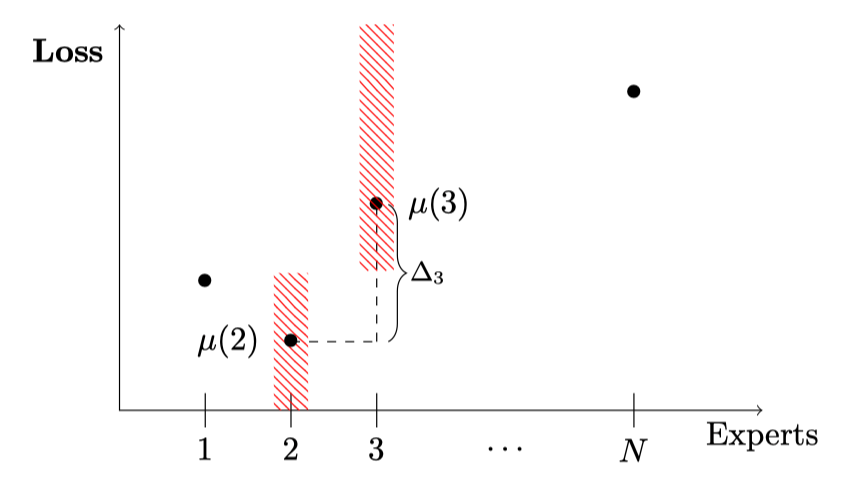
\includegraphics[width=0.7\textwidth]{Figs/5.png}
    \caption{The case in the proof of \cref{thm:fsdddea4q} where $a=3, a^{*}=2$, and neither $E_{1}$ or $E_{2}$ happens. Then $\hat{\mu}_{T_{0}}(2)$ and $\hat{\mu}_{T_{0}}(3)$ lie in the shaded red regions.}
    \label{fig:eezcvsafd}
\end{figure}
\begin{proof}
The proof uses Hoeffding's inequality to show that for actions $a$ with $\mu(a)>\mu\left(a^{*}\right)$, we also have $\hat{\mu}_{T_{0}}(a)>\hat{\mu}_{T_{0}}\left(a^{*}\right)$ with high probability (depending on $T_{0}$ ).

We have
\begin{align*}
\operatorname{ Regret }_{\mathrm{stoch }}=\sum_{a \in[N]} \Delta_{a} \mathbb{E}\left(n_{t}(a)\right)
\end{align*}
Therefore it suffices to bound
\begin{align*}
\mathbb{E}\left(n_{T}(a)\right) \leq \frac{T_{0}}{N}+2 T \exp \left(\frac{-T_{0} \Delta_{a}^{2}}{8 N}\right)
\end{align*}
for each action $a$ with $\Delta_{a}>0$
For any action $a$, notice that at the end of the explore phase $\hat{\mu}_{T_{0}}(a)$ is an average of $T_{0} / N$ i.i.d. draws $\ell_{i}(a) \in[0,1] .$ By Hoeffding's inequality,
\begin{align*}
\begin{gathered}
P \underbrace{\left(\mu(a)-\hat{\mu}_{T_{0}}(a) \geq \frac{\Delta_{a}}{2}\right)}_{E_{1}} \leq \exp \left(-\frac{T_{0} \Delta_{a}^{2}}{8 N}\right) \\
P \underbrace{\left(\hat{\mu}_{T_{0}}\left(a^{*}\right)-\mu\left(a^{*}\right) \geq \frac{\Delta_{a}}{2}\right)}_{E_{2}} \leq \exp \left(-\frac{T_{0} \Delta_{a}^{2}}{8 N}\right)
\end{gathered}
\end{align*}
Suppose neither event $E_{1}$ or event $E_{2}$ happens. Then $\hat{\mu}_{T_{0}}(a)>\hat{\mu}_{T_{0}}\left(a^{*}\right) .$ (See Figure
\cref{fig:eezcvsafd}) As a result, the algorithm never plays action $a$ for any time $t$ during the \tb{exploit phase}. Thus $n_{T}(a)=\frac{T_{0}}{N}$ and therefore $\mathbb{E}\left(n_{T}(a) \mid E_{1}^{c} \cap E_{2}^{c}\right) \leq \frac{T_{0}}{N}$.

Also
\begin{align*}
\begin{aligned}
P\left(E_{1}^{c} \cap E_{2}^{c}\right) & \leq 1 \\
\mathbb{E}\left(n_{T}(a) \mid E_{1} \cup E_{2}\right) & \leq T \\
P\left(E_{1} \cup E_{2}\right) & \leq 2 \exp \left(-\frac{T_{0} \Delta_{a}^{2}}{8 N}\right)
\end{aligned}
\end{align*}
so by the law of total expectation
\begin{align*}
\mathbb{E}\left(n_{T}(a)\right) \leq \frac{T_{0}}{N}+2 T \exp \left(\frac{-T_{0} \Delta_{a}^{2}}{8 N}\right)
\end{align*}
as required.
\end{proof}
\begin{rema}\bfs{drawback of the Explore-Then-Exploit algorithm}
  It wastes time exploring bad actions during the explore phase, and potentially misses out on better actions during the exploit phase (big variance). In the next section, we cover the UCB algorithm, which balances exploration and exploitation at each step.
\end{rema}
\subsubsection{The UCB Algorithm}
$\bullet$ \tb{Key:}
\begin{itemize}
    \item It takes into account how confident the player is in the estimate $\hat{\mu}_{t}(a)$. The algorithm builds a \tb{confidence interval} $I_{t}=\left[x_{a, t}, y_{a, t}\right]$ around $\hat{\mu}_{t}(a)$ so that $\mu(a)$ lies in $I_{t}$ with high probability. 
    \item It then picks $a_{t}=\argmin_{a \in[N]} x_{a, t}$ at each step. 
    \item This setup allows UCB to \tb{explore and exploit simultaneously}:

 For little-explored actions, the interval $I_{t}$ will be large. This encourages exploration because the player is incentivized to pick $a$ since the lower bound $x_{a, t}$ will be small (relative to $\hat{\mu}_{t}(a)$ ). At the same time, the algorithm avoids wasting excessive time on actions with large values of $\mu(a)$. And UCB exploits its information at each step by picking $a_{t}=\argmin_{a \in[N]} x_{a, t} .$
\end{itemize}
\begin{rema}
  The reason the algorithm is called "Upper" Confidence Bound and not "Lower" Confidence Bound is because in the literature researchers focus on maximizing reward whereas in our problem we minimize loss.
\end{rema}

\begin{lema}
  Fix an action a in $[N]$. With probability $1-\frac{1}{T}$ we have
\begin{align*}
\mu(a) \in\left[\hat{\mu}_{t}(a)-2\sqrt{\frac{\log (T)}{n_{t}(a)}}, \hat{\mu}_{t}(a)+2\sqrt{\frac{\log (T)}{n_{t}(a)}}\right]
\end{align*}
for each $t=1, \ldots, T.$
\end{lema}
\begin{proof}
Suppose we have random selected the arm $a$ for $n$ times,  by Hoeffding's inequality with probability $1-2 \exp \left(-2 c^{2}\right)$ we have
\begin{align*}
\left|\frac{\sum_i \ell_i(a)}{t}-\mu(a)\right| \leq \frac{c}{\sqrt{n}}
\end{align*}
Plugging in $c=\sqrt{\log (T)}$, we get that with probability $1-\frac{2}{T^{2}}$, we get
\begin{align*}
\left|\frac{\sum_i \ell_i(a)}{t}-\mu(a)\right| \leq \sqrt{\frac{\log (T)}{t}}
\end{align*}
Taking a \tb{union bound} over $t=1, \ldots, T$, we get that with  with probability $1-\frac{2}{T}$,
\begin{align*}
\left|\frac{\sum_i \ell_i(a)}{t}-\mu(a)\right| \leq \sqrt{\frac{\log (T)}{t}} \quad \forall t\in [T]
\end{align*}
We then substitute a random variable $n_t(a)\in [T]$ with probability $1$ and get with probability $1-\frac{2}{T}$,
\begin{align*}
\left|\frac{\sum_{i=1}^{n_t(a)} \ell_i(a)}{n_t(a)}-\mu(a)\right| \leq \sqrt{\frac{\log (T)}{n_t(a)}}.
\end{align*}
Note here $n_t(a)$ can be dependent on $\ell_i(a)$. It is okay for $n_t(a)$ to have any distribution as long as $n_t(a)\in [T]$ with probability $1$.

Note $\hat{\mu}_{t}(a) \triangleq \frac{1}{n_{t}(a)} \sum_{i=1}^{t} \ell_{i}(a) \indicator{a_{i}=a}= \frac{\sum_{i=1}^{n_t(a)} \ell_i(a)}{n_t(a)}$ because $\ell_{i}(a)$ are independent, and  $\indicator{a_{i}=a}$ and $\ell_{i}(a)$ are independent (but $n_{t}(a)$ and  $\ell_{i}(a)$ are not independent due to the algorithm process).

Note here for convenience of further regret proof, we use $1-\frac{1}{T}$.
\end{proof}
\begin{rema}
The strong conclusion is from the uniform bound, please also see "Supervised Learning" Remark 3.4 for more explanation. Maybe you can better understand the union bound by writing it as
\begin{align*}
\operatorname{Pr}\left(\sup_{t\in [T]} \left|\frac{\sum_i \ell_i(a)}{t}-\mu(a)\right| \leq \sqrt{\frac{\log (T)}{t}}\right) \ge 1-\frac{2}{T}
\end{align*} 
\end{rema}

We are ready to state the UCB algorithm. Define the lower confidence bound $\operatorname{LCB}_{t}(a)$ at time $t$:
\begin{align*}
\operatorname{LCB}_{t}(a) \triangleq \hat{\mu}_{t-1}(a)-2\sqrt{\frac{\log (T)}{n_{t-1}(a)}}
\end{align*}
$\bullet$ \tb{ UCB algorithm (“optimism in the face of uncertainty):}

\boxx{
At each step $t$, the player picks the action $\argmin_{a \in[N]}\mathrm{LCB}_{t}(a)$.}
\paragraph{Bounding the Regret}
\begin{thma}
The regret of the UCB algorithm is bounded above by
\begin{align*}
\sum_{a: \Delta_a>0} O\left(\frac{\log T}{\Delta_a}\right)
\end{align*}
\end{thma} 
\begin{rema}
In comparison, the explore-then-exploit algorithm has regret $\sum O\left(\frac{\log T \cdot \Delta_a}{\Delta^{2}}\right)\ge \sum_{a: \Delta_a>0} O\left(\frac{\log T}{\Delta_a}\right).$
\end{rema}The proof is pretty straighforward given the earlier claim:
\begin{proof}
Recall that the regret is equal to
\begin{align*}
\sum\left[n_{T}(a)\right] \cdot \Delta_a
\end{align*}

Thus it suffices to show that $\mathbb{E}\left[n_{T}(a)\right] \geq O\left(\frac{\log T}{\Delta_a^{2}}\right)$ for all $a$. Fix one such $a$. We define $T_{0}$ analogously in the explore-and-exploit algorithm:
\begin{align*}
T_{0} \triangleq \frac{20 \log T}{\Delta_a^{2}}
\end{align*}
We have 
$$
 \mathbb{E}\left[n_{T}(a)\right] \leq T_{0}+\sum_{t=T_{0}}^{T} \mathbb{E}\left[\mathbf{1}\left(a_{t}=a, n_{t-1}(a) \geq T_{0}\right)\right].
$$
This is because
\begin{align*}
\begin{aligned}
\mathbb{E}\left[n_{T}(a)\right] &=\mathbb{E}\left[\sum_{t=1}^{T} \mathbf{1}\left(a_{t}=a\right)\right] \\
&=\sum_{t=1}^{T} \mathbb{E}\left[\mathbf{1}\left(a_{t}=a, n_{t-1}(a)<T_{0}\right)\right]+\sum_{t=1}^{T} \E\left[\mathbf{1}\left(a_{t}=a, n_{t-1}(a) \geq T_{0}\right)\right]
\end{aligned}
\end{align*}
Define:
\begin{itemize}
    \item $E_{a}$: $\hat{\mu}_{t-1}(a) \geq \mu(a)-2 \sqrt{\frac{\log T}{n_{t-1}(a)}}$
    \item $E_{a^{*}}$:$\hat{\mu}_{t-1}(a^*) -2 \sqrt{\frac{\log T}{n_{t-1}(a^*)}} \le \mu(a^*)$
\end{itemize}
Suppose the events $E_{a}, E_{a^{*}}$ in the claim happen. Then
\begin{align*}
\begin{aligned}
\operatorname{LCB}_{t}\left(a^{*}\right) & \leq \mu\left(a^{*}\right) \\
\operatorname{LCB}_{t}(a) &=\hat{\mu}_{t-1}(a)-2 \sqrt{\frac{\log T}{n_{t-1}(a)}} \\
& \geq \mu(a)-2 \sqrt{\frac{\log T}{n_{t-1}(a)}}-2 \sqrt{\frac{\log T}{n_{t-1}(a)}} \\
& \geq \mu\left(a^{*}\right)+\Delta_a-4 \sqrt{\frac{\log T}{n_{t-1}(a)}} \\
& \geq \mu\left(a^{*}\right)+\Delta_a-4 \sqrt{\frac{\log T}{T_{0}}} \\
&>\mu\left(a^{*}\right)
\end{aligned}
\end{align*}
Hence $\operatorname{LCB}_{t}(a) \geq \operatorname{LCB}_{t}\left(a^{*}\right)$ and $a_{t} \neq a$. Therefore
\begin{align*}
\begin{aligned}
\mathbb{E}\left[n_{T}(a)\right] & \leq T_{0}+\sum_{t=1}^{T} \operatorname{Pr}\left[E_{a}^c \cup E_{a^{*}}^c\right] \\
& \leq T_{0}+\frac{2}{T}\left(T-T_{0}\right) \\
& \leq T_{0}+2 \leq 2 T_{0} \leq O\left(\frac{\log T}{\Delta_a^{2}}\right)
\end{aligned}
\end{align*}
\end{proof}

\subsection{Stochastic Bayesian Setting}
Before going, I would like to explain a little bit about frequentist vs Bayesian:

\emph{It is often said (\tb{incorrectly}) that ‘parameters are treated as fixed by the frequentist but as random by the Bayesian’. For frequentists and Bayesians alike, the value of a parameter may have been fixed from the start or may have been generated from a physically random mechanism. \tb{In either case, both suppose it has taken on some fixed value that we would like to know.} The Bayesian uses formal probability models to express personal uncertainty about that value. The ‘randomness’ in these models represents personal uncertainty about the parameter’s value; it is not a property of the parameter (although we should hope it accurately reflects properties of the mechanisms that produced the parameter).}

\subsubsection{Setup}
$\bullet$ \tb{Assumption:}
\begin{itemize}
    \item Let $\Theta$ be the \tb{model parameter} space and $\theta^{*}$ the ground truth model parameter. Furthermore, let $Q$ be the \tb{prior distribution} of $\theta^{*}$, i.e., $\theta^{*} \sim Q$. Unless otherwise stated, we assume $\Theta$ to be a finite set.
    (In the stochastic non-Bayesian setting, this was $\mu(1), \ldots, \mu(N)$.)
    \item Let $\mathcal{A}$ be the \tb{action space}. Unless otherwise stated, we assume $\mathcal{A}$ to be a finite set.
    (In the stochastic non-Bayesian setting, this was $\in[N]$.)
    \item  Let $D(a, \theta)$ be the \tb{distribution of loss} for $a \in \mathcal{A}$ and for a particular $\theta \in \Theta$. (In  the stochastic non-Bayesian setting,  this was $D_{a}$.)
    \item At iteration $t$, if action $A_{t}$ is played, we observe the loss $L_{A_{t}, \theta^{*}} \sim D\left(A_{t}, \theta^{*}\right)$. For notational ease, we define $$L_{t} \triangleq L_{A_{t}, \theta^{*}}.$$ The uppercase notation of $A_{t}$ emphasizes that $A_{t}$ is a random variable.
    \item The optimal action is a function $a^{*}: \Theta \rightarrow \mathcal{A}$ defined as
\begin{align*}
a^{*}(\theta)=\underset{a \in \mathcal{A}}{\operatorname{argmin}} \underset{L \sim D(a, \theta)}{\mathbb{E}}[L]
\end{align*}
With this, we also define the optimal action at the ground truth parameter
\begin{align*}
A^{*}=a^{*}\left(\theta^{*}\right)
\end{align*}
\item Let $A_{1}, \ldots, A_{T}$ be the actions played at iterations $1, \ldots, T$. Define the regret as
\begin{align*}
\re=\sum_{t=1}^{T} \mathbb{E}\left[L_{t}-L_{A^{*}, \theta^{*}}\right]
\end{align*}
where the expectation is taken over all the random variables. In the Bayesian setting, the ground truth parameter $\theta^{*}$, the actions $A_{1}, \ldots, A_{T}$, and the losses $L_{A^{*}, \theta^{*}}, L_{1}, \ldots, L_{T}$ are all random variables.
\end{itemize}
\begin{rema}\bfs{more explanation for the regret}
For a ground truth $\theta^{*}$ and actions $a_{1}, \ldots, a_{T}$, we define
\begin{align*}
\operatorname{Regret}\left(\theta^{*}, a, \ldots, a_{T}\right)=\underset{L_{a_{t}, \theta^{*}} \sim D\left(a_{t}, \theta^{*}\right) ; L_{a_{t}^{*}, \theta^{*}} \sim D\left(a^{*}\left(\theta^{*}\right), \theta^{*}\right)}{\mathbb{E}}\left[\sum_{t} L_{a_{t}, \theta^{*}}-\sum_{t} L_{a^{*}\left(\theta^{*}\right), \theta^{*}}\right]
\end{align*}
In the Bayesian setting,  $\theta^{*}$ is posited to be drawn from some distribution $Q$. Let $A_{1}, \ldots, A_{T}$ be the (possible random) actions taken by the algorithm. Then the Bayesian regret of the algorithm is defined as follows:
\begin{align*}
\re=\underset{\theta^{*} \sim Q}{\mathbb{E}}\left[\underset{A_{1}, \ldots, A_{T}}{\mathbb{E}}\left[\operatorname{Regret}\left(\theta^{*}, A_{1}, \ldots, A_{T}\right)\right]\right]
\end{align*}
\end{rema}

\subsubsection{Thompson Sampling Algorithm}
$\bullet$ \tb{Explore-Then-Exploit Algorithm:}

\boxx{
At iteration $t$, the algorithm proceeds as:
\begin{enumerate}
    \item Define $f_{t-1}$ as the collection of random variables observed so far. That is
\begin{align*}
f_{t-1}=\left\{A_{1}, L_{1}, \ldots, A_{t-1}, L_{t-1}\right\}
\end{align*}
\item Compute
\begin{align*}
P_{t}(\theta)=\operatorname{Pr}\left(\theta^{*}=\theta \mid f_{t-1}\right)
\end{align*}
which is the posterior distribution of $\theta^{*} \mid f_{t-1}$.
\item Sample $\theta_{t}$ from $P_{t}$.
\item Play the action $a^{*}\left(\theta_{t}\right)$.
\end{enumerate}
}

\subsubsection{Bounding the Regret}
We will use information theory to provide a regret bound for Thompson sampling. 

$\bullet$ \tb{proof steps:}
\begin{enumerate}
    \item First, we define the notion of \tb{information ratio}, 
    \item Second, we show that bounding the information ratio implies bounding the regret.
    \item Third, we provide a bound for the information ratio, thereby bounding the regret.
    \item Finally, we apply these results to bound the regret for the \tb{multi-armed bandit problem} and \tb{linear bandit problem} in the Bayesian setting.
\end{enumerate}
\paragraph{Information Ratio}
\begin{defa}\bfs{Information Ratio}
 The information ratio at iteration $t$ is
\begin{align*}
\Gamma_{t}=\frac{\big[\mathbb{E}\left[L_{t}-L_{A^{*}, \theta^{*}} \mid f_{t-1}\right]\big]^{2}}{I\left(A^{*} ;\left(A_{t}, L_{t}\right) \mid f_{t-1}\right)},
\end{align*}
where $I$ is the mutal information.
\end{defa}
\begin{rema}
The numerator is the square of the regret term at iteration $t$, which is a random variable. The denominator is the conditional mutual information between the optimal action $A^{*}$ and $\left(A_{t}, L_{t}\right)$, conditioned on the previously observed actions and losses. Note that the denominator is a \tb{scalar} (not random).
\end{rema} 
\begin{rema}\bfs{explanation}
Intuitively, the \tb{denominator is the amount of information gained about $A^{*}$ from observing $A_{t}$ and $L_{t}$.} Therefore, a small information ratio is desirable. With a small information ratio, if an algorithm suffers a lot of regret, it also gains more information about the optimal action.
\end{rema} 
\paragraph{Regret Bounds Using Information Ratio}
\begin{thma}\bfs{regret bounds using information ratio}\label{thm:hdafrw}
If for all $t=1, \ldots, T, \Gamma_{t} \leq \Gamma$ almost surely for some constant $\Gamma$, then
\begin{align*}
\re \leq \sqrt{\Gamma \cdot H\left(A^{*}\right) \cdot T}
\end{align*}
\end{thma}
\begin{rema}\bfs{explanation}
This theorem shows that the regret can be bounded based on a bound on the \tb{information ratio}. 
\end{rema}
\begin{proof}
\begin{align*}
\re &=\sum_{t=1}^{T} \mathbb{E}\left[L_{t}-L_{A^{*}, \theta^{*}}\right]\nn
&=\sum_{t=1}^{T} \underset{f_{t-1}}{\mathbb{E}}\left[\mathbb{E}\left[L_{t}-L_{A^{*}, \theta^{*}} \mid f_{t-1}\right]\right] \text { (law of total expectation) }\nn
& \leq \sum_{t=1}^{T} \underset{f_{t-1}}{\mathbb{E}}\left[\Gamma^{\frac{1}{2}} \cdot I\left(A^{*} ;\left(A_{t}, L_{t}\right) \mid f_{t-1}\right)^{\frac{1}{2}}\right]\text { (definition of  $\Gamma_{t}$, and  $\Gamma_{t} \leq \Gamma$)}\nn
& \leq \Gamma^{\frac{1}{2}} \sum_{t=1}^{T}\bigg[\mathbb{E}\left[I\left(A^{*} ;\left(A_{t}, L_{t}\right) \mid f_{t-1}\right)\right]\bigg]^{\frac{1}{2}}\text { (Cauchy-Schwarz or Jensen inequality)}\nn
& \leq \Gamma^{\frac{1}{2}} \cdot T^{\frac{1}{2}}\left(\sum_{t=1}^{T} \mathbb{E}\left[I\left(A^{*} ;\left(A_{t}, L_{t}\right) \mid f_{t-1}\right)\right]\right)^{\frac{1}{2}} \text { (Cauchy-Schwarz or Jensen ($\frac{1}{T}$ as distribution) inequality)}\\
&=\Gamma^{\frac{1}{2}} \cdot T^{\frac{1}{2}}\left(\sum_{t=1}^{T} I\left(A^{*} ;\left(A_{t}, L_{t}\right) \mid f_{t-1}\right)\right)^{\frac{1}{2}} \text { (the mutual information is a scalar) }\nn
&=\Gamma^{\frac{1}{2}} \cdot T^{\frac{1}{2}} \cdot I\left(A^{*} ;\left(A_{1}, L_{1}, \ldots, A_{T}, L_{T}\right)\right)^{\frac{1}{2}} \text { (chain rule) }\nn
&\leq \Gamma^{\frac{1}{2}} \cdot T^{\frac{1}{2}} \cdot H\left(A^{*}\right)^{\frac{1}{2}}
\end{align*}
where $H$ is the entropy.
\end{proof}
\paragraph{Bounds for Information Ratio}
We will then discuss two lemmas that lead to a useful bound on the information ratio. For the remaining exposition, we simplify the notations in the following way (subscript $t$ may be omitted): 
% \centerline{let $p_{t}$ be the distribution of $\theta^{*} \mid f_{t-1}$, and $q_{t}$ be the distribution of $A^{*} \mid f_{t-1} $.}
\begin{align*}
    p_{t}&=\operatorname{Pr}(\theta^{*} \mid f_{t-1})\\
     q_{t}&=\operatorname{Pr}(A^{*} \mid f_{t-1})
\end{align*}
$\bullet$ \tb{insight}:

Recall that in Thompson sampling, the algorithm computes $p_{t}$, draws $\theta_{t}$ from $p_{t}$, and sets $A_{t}=a^{*}\left(\theta_{t}\right)$ (all of these are conditioned on $f_{t-1}$ ). Therefore, $A_{t} \mid f_{t-1}$ has the same distribution as $q_{t}$. It follows that $A_{t} \mid f_{t-1}$ and $A^{*} \mid f_{t-1}$ are \tb{identically and independently distributed.}


\begin{lema}
  Assume $L_{a, \theta} \in[0,1]$ almost surely for all $a \in \mathcal{A}, \theta \in \Theta$. Suppose $A^{*}$ follows the distribution $q$, and $A \sim q$ is independent from $A^{*} .$ Let $L \sim D\left(A, \theta^{*}\right)$ where $\theta^{*} \sim p .$ Define the matrix $M \in \mathbb{R}^{|\mathcal{A}| \times|\mathcal{A}|}$ as
\begin{align*}
M_{a, a^{\prime}}=\sqrt{q(a) q\left(a^{\prime}\right)} \cdot\bigg[\mathbb{E}\left[L_{a, \theta^{*}} \mid A^{*}=a^{\prime}\right]-\mathbb{E}\left[L_{a, \theta^{*}}\right]\bigg]
\end{align*}
Then
\begin{align*}
I\left(A^{*} ;(A, L)\right) \geq\|M\|_{F}^{2}
\end{align*}
\end{lema} 
\begin{rema}\label{lem:iaerad}
It is complicated to understand, please see the proof for intuition.
\end{rema}
\begin{proof}
\begin{align*}
\begin{aligned}
I\left(A^{*} ;(A, L)\right) &=I\left(A^{*} ; L \mid A\right)+I\left(A^{*} ; A\right) \text { (chain rule) } \\
&=I\left(A^{*} ; L \mid A\right)\text { ($A^{*}$ and  $A$ are independent)} \\
&=\sum_{a \in \mathcal{A}} q(a) I\left(A^{*} ; L \mid A=a\right) \text { (definition) } \\
&=\sum_{a \in \mathcal{A}} q(a) I\left(A^{*} ; L_{a, \theta^{*}}\right)\left(A^{*} \text { and } A \text { are independent; } L_{A, \theta^{*}} \sim D\left(A, \theta^{*}\right)\right) \\
&=\sum_{a \in \mathcal{A}} q(a) \sum_{a^{\prime} \in \mathcal{A}} q\left(a^{\prime}\right) \operatorname{KL}\left(P_{L_{a, \theta^{*} \mid A^{*}=a^{\prime}}} \| P_{L_{a, \theta^{*}}}\right) \text { (See Tay's information notes) } \\
& \geq \sum_{a \in \mathcal{A}} q(a) \sum_{a^{\prime} \in \mathcal{A}} q\left(a^{\prime}\right) \operatorname{TV}\left(P_{L_{a, \theta^{*} \mid A^{*}=a^{\prime}}}, P_{L_{a, \theta^{*}}}\right)^{2} \text { (Pinsker inequality) }
\end{aligned}
\end{align*}

\end{proof}
Recall that $\operatorname{TV}(p, q)=\sup_{f \leq 1}\left|\mathbb{E}_{p} f-\mathbb{E}_{q} f\right| .$ Taking $f(x)=x\in[0,1]$ ($f=0$, otherwise) in
\begin{align*}
\operatorname{TV}\left(P_{L_{a, \theta^{*} \mid A^{*}=a^{\prime}}}, P_{L_{a, \theta^{*}}}\right)
\end{align*}
gives us a lower bound on the TV. It follows that
\begin{align*}
\begin{aligned}
I\left(A^{*} ;(A, L)\right) & \geq \sum_{a \in \mathcal{A}} q(a) \sum_{a^{\prime} \in \mathcal{A}} q\left(a^{\prime}\right)\bigg[\mathbb{E}\left[L_{a, \theta^{*}} \mid A^{*}=a\right]-\mathbb{E}\left[L_{a, \theta^{*}}\right]\bigg]^{2} \\
&=\|M\|_{F}^{2}
\end{aligned}
\end{align*}

\begin{lema}
  In the same setting as \cref{lem:iaerad},
\begin{align*}
\mathbb{E}\left[L_{A, \theta^{*}}-L_{A^{*}, \theta^{*}}\right]=-\operatorname{trace}(M)
\end{align*}
\end{lema}
\begin{proof}
Recall that $M_{a, a^{\prime}}=\sqrt{q(a) q\left(a^{\prime}\right)} \cdot\left[\mathbb{E}\left[L_{a, \theta^{*}} \mid A^{*}=a^{\prime}\right]-\mathbb{E}\left[L_{a, \theta^{*}}\right]\right]$
\begin{align*}
\operatorname{trace}(M) &=\sum_{a \in \mathcal{A}} M_{a, a} \\
&=\sum_{a \in \mathcal{A}} \sqrt{q(a) q(a)} \cdot\bigg[\mathbb{E}\left[L_{a, \theta^{*}} \mid A^{*}=a\right]-\mathbb{E}\left[L_{a, \theta^{*}}\right]\bigg] \\
&=\sum_{a \in \mathcal{A}} q(a) \cdot\bigg[\mathbb{E}\left[L_{a, \theta^{*}} \mid A^{*}=a\right]-\mathbb{E}\left[L_{a, \theta^{*}}\right]\bigg] \\
&=\underset{a \sim q}{\mathbb{E}}\bigg[\mathbb{E}\big[L_{a, \theta^{*}} \mid A^{*}=a\big]\bigg]-\underset{a \sim q}{\mathbb{E}}\bigg[\mathbb{E}\left[L_{a, \theta^{*}}\right]\bigg] \\
&=\mathbb{E}\left[L_{A^{*}, \theta^{*}}-L_{A, \theta^{*}}\right]
\end{align*}

\end{proof}

\begin{cora}
  In the same setting as \cref{lem:iaerad},the information ratio is upper bounded by $\operatorname{rank}(M)$
  \end{cora} 
  \begin{proof}
  We have the information ratio
\begin{align*}
\frac{\left[\mathbb{E}\left[L_{A, \theta^{*}}-L_{A^{*}, \theta^{*}}\right]\right]^{2}}{I\left(A^{*} ;(A, L)\right)} \leq \frac{\operatorname{trace}(M)^{2}}{\|M\|_{F}^{2}} \leq \operatorname{rank}(M)
\end{align*}
\end{proof}
\paragraph{Final Regret Bounds}
We now apply the results to bound the regret of specific problems.

$\bullet$ \tb{multi-armed bandit problem:}
\begin{cora}
  Assume that the loss is bounded between 0 and $1 .$ For the multi-armed bandit problem, we have the regret bound
\begin{align*}
\re \leq \sqrt{T \cdot|\mathcal{A}| \cdot \log |\mathcal{A}|}
\end{align*}
\end{cora} 
\begin{proof}
The information ratio is upper bounded by $\operatorname{rank}(M)$, which is bounded by $|\mathcal{A}|$. By Fact $1, H\left(A^{*}\right) \leq \log |\mathcal{A}| .$ Applying these to \cref{thm:hdafrw} gives the desired bound.
\end{proof} 

$\bullet$ \tb{linear bandit problem:}
\begin{cora}
  Assume that the loss is bounded between 0 and 1 . For the linear bandit problem with $\theta \in \mathbb{R}^{d}, a \in \mathbb{R}^{d}$ such that $\|\theta\|_{2} \leq 1,\|a\|_{2} \leq 1$, we have the regret bound
\begin{align*}
\re\leq d \sqrt{T \log T}
\end{align*}
\end{cora} 
Proof. We have $\operatorname{rank}(M) \leq d$. Consider the $\epsilon$-cover of the $L_{2}$ unit ball. Setting $\epsilon=1 / O(T)$, we have
\begin{align*}
\begin{aligned}
|\mathcal{A}| & \leq O(T)^{d} \\
\Rightarrow H\left(A^{*}\right) & \leq d \log T
\end{aligned}
\end{align*}
Applying these to \cref{thm:hdafrw} gives the desired bound.

\bibliographystyle{IEEEtran}
\bibliography{IEEEabrv,StringDefinitions,adv_dnn}

\end{document}